\documentclass[11pt]{article}
\usepackage[textwidth=18.0cm, textheight=23.0cm, top=2.0cm]{geometry}
\usepackage{pst-all}
\usepackage{amssymb}
\usepackage{tikz}
\usepackage{underscore}\begin{document}
\pagestyle{empty}


ClassName: \underline{\textbf{Class_07.2bp-32}}
\par
BinSize: \underline{\textbf{100 × 100}}
\par
ReduceSize: \underline{\textbf{100 × 100}}
\par
TypeNum: \underline{\textbf{80}}
\par
Num: \underline{\textbf{80}}
\par
OutS: \underline{\textbf{210000}}
\par
InS: \underline{\textbf{177250}}
\par
Rate: \underline{\textbf{0.844}}
\par
UB: \underline{\textbf{21}}
\par
LB0: \underline{\textbf{20}}
\par
LB: \underline{\textbf{21}}
\par
LBWithCut: \underline{\textbf{21}}
\par
NodeCut: \underline{\textbf{0}}
\par
ExtendedNodeCnt: \underline{\textbf{1}}
\par
GenNodeCnt: \underline{\textbf{1}}
\par
PrimalNode: \underline{\textbf{0}}
\par
ColumnCount: \underline{\textbf{93}}
\par
TotalCutCount: \underline{\textbf{0}}
\par
RootCutCount: \underline{\textbf{0}}
\par
LPSolverCnt: \underline{\textbf{73}}
\par
PricingSolverCnt: \underline{\textbf{73}}
\par
BranchAndBoundNum: \underline{\textbf{1}}
\par
isOpt: \underline{\textbf{false}}
\par
TimeOnInitSolution: \underline{\textbf{600.000 s}}
\par
TimeOnPrimal: \underline{\textbf{0.000 s}}
\par
TimeOnPricing: \underline{\textbf{2999.608 s}}
\par
TimeOnRmp: \underline{\textbf{0.113 s}}
\par
TotalTime: \underline{\textbf{3600.004 s}}
\par
\newpage


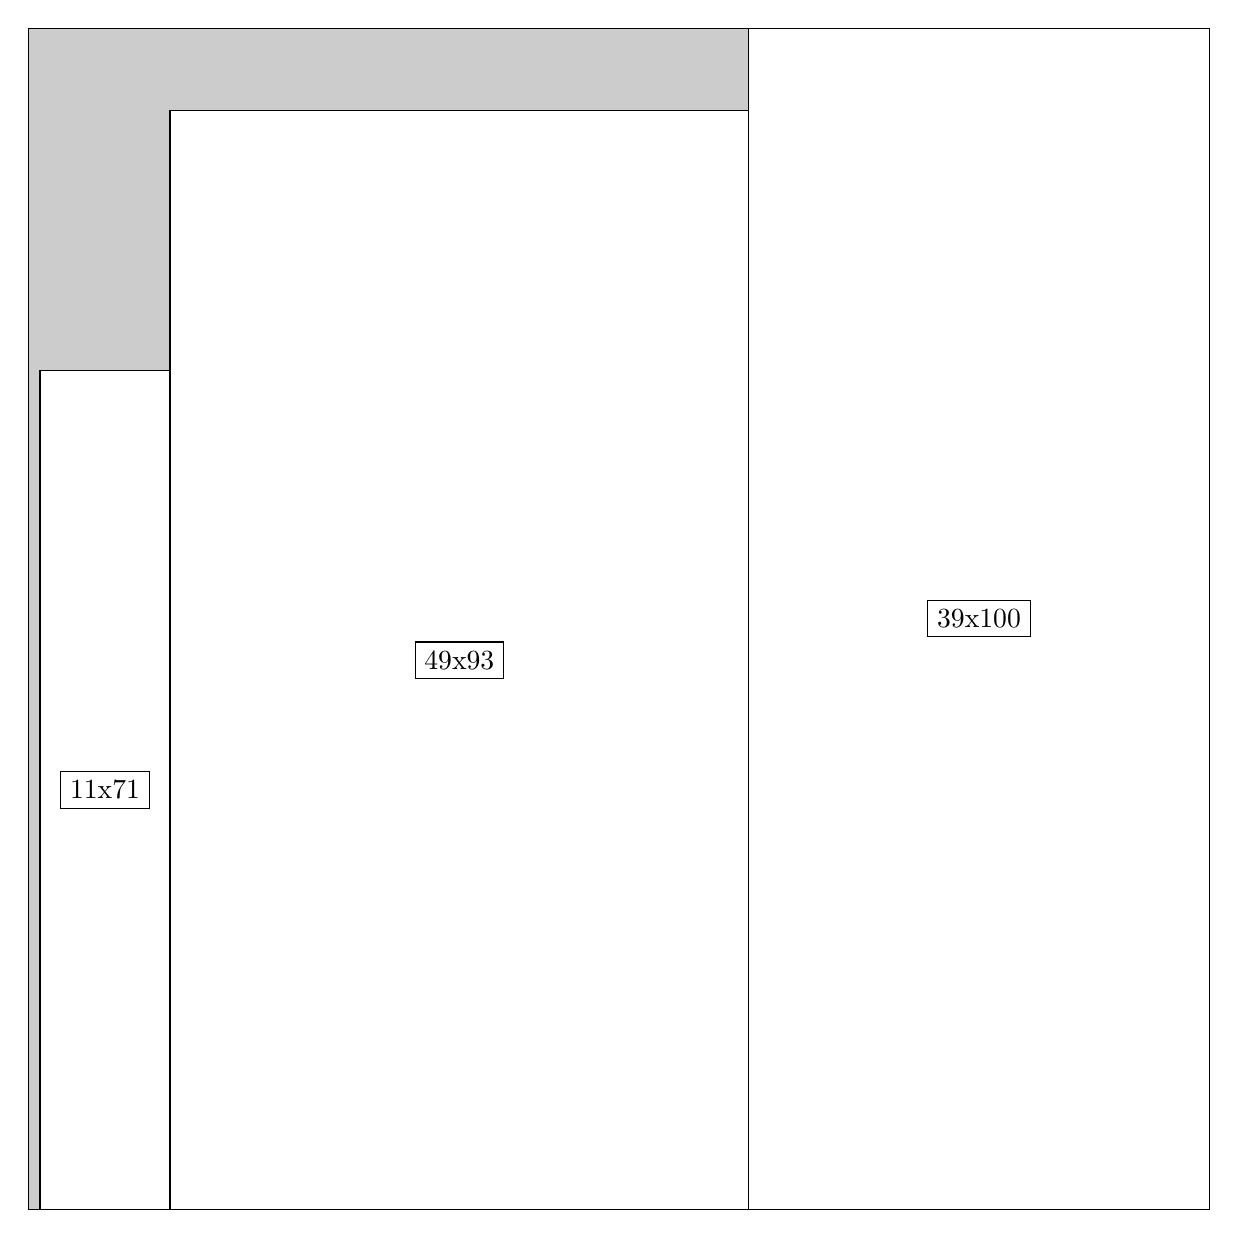
\begin{tikzpicture}[shorten >=1pt,scale=1.0,every node/.style={scale=1.0},->]
\tikzstyle{vertex}=[circle,fill=black!25,minimum size=14pt,inner sep=0pt]
\filldraw[fill=gray!40!white, draw=black] (0,0) rectangle (15.0,15.0);
\foreach \name/\x/\y/\w/\h in {39x100/9.15/0.0/5.85/15.0,49x93/1.7999999999999998/0.0/7.35/13.95,11x71/0.15/0.0/1.65/10.65}
\filldraw[fill=white!40!white, draw=black] (\x,\y) rectangle node[draw] (\name) {\name} ++(\w,\h);
\end{tikzpicture}


w =39 , h =100 , x =61 , y =0 , v =3900
\par
w =49 , h =93 , x =12 , y =0 , v =4557
\par
w =11 , h =71 , x =1 , y =0 , v =781
\par
\newpage


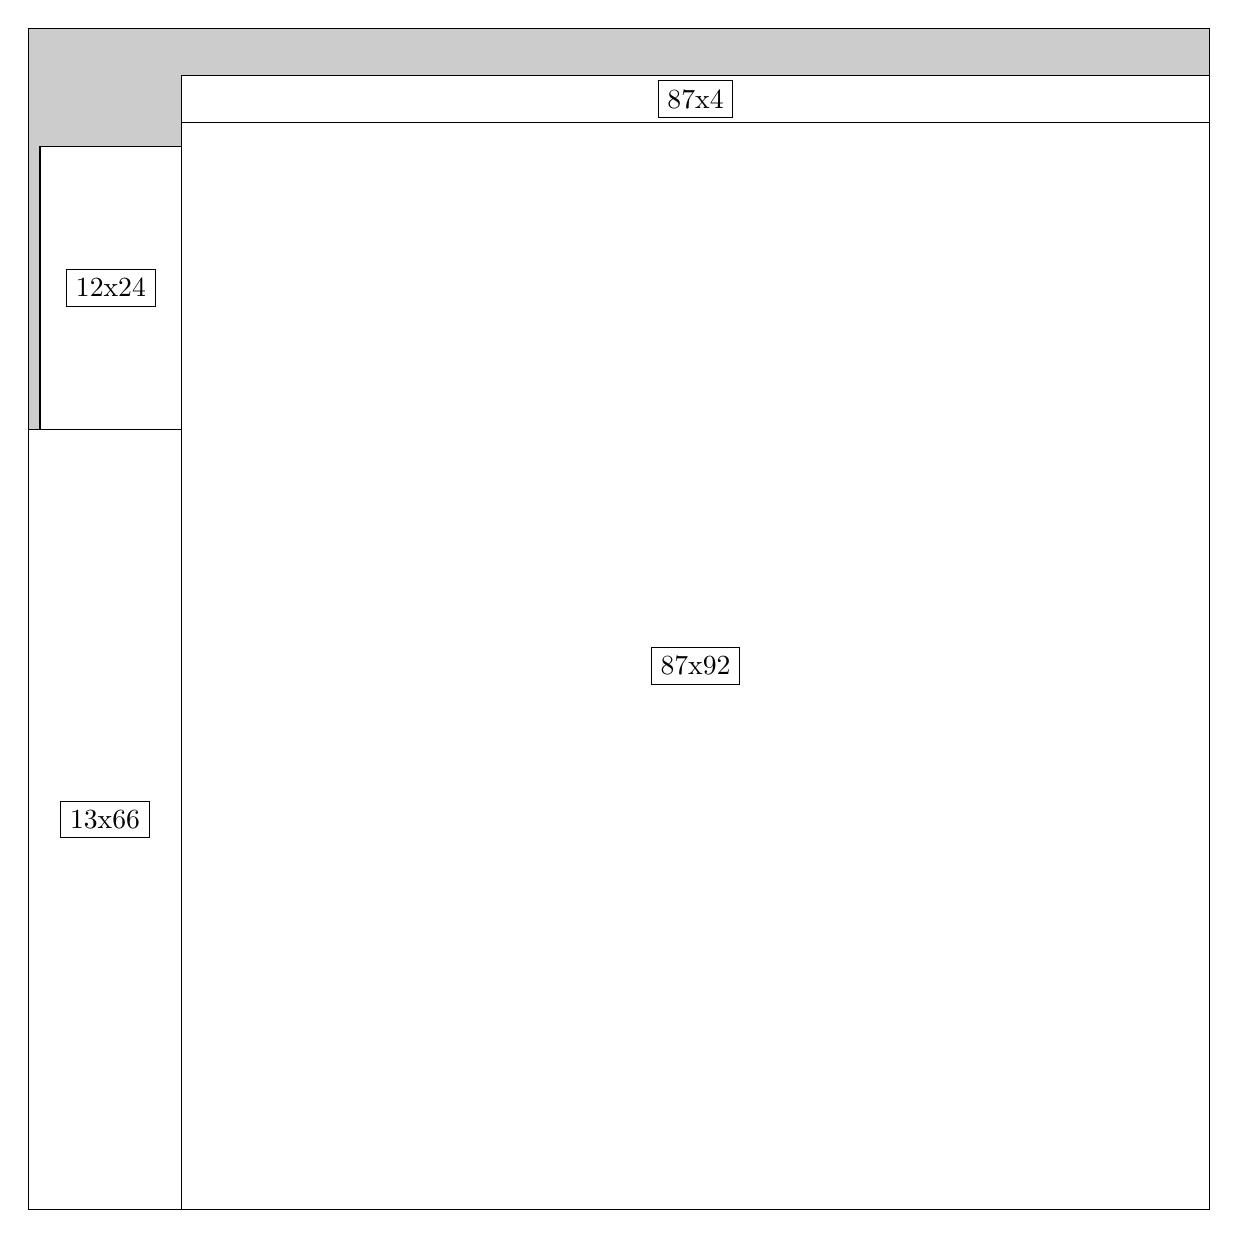
\begin{tikzpicture}[shorten >=1pt,scale=1.0,every node/.style={scale=1.0},->]
\tikzstyle{vertex}=[circle,fill=black!25,minimum size=14pt,inner sep=0pt]
\filldraw[fill=gray!40!white, draw=black] (0,0) rectangle (15.0,15.0);
\foreach \name/\x/\y/\w/\h in {87x92/1.95/0.0/13.049999999999999/13.799999999999999,13x66/0.0/0.0/1.95/9.9,12x24/0.15/9.9/1.7999999999999998/3.5999999999999996,87x4/1.95/13.799999999999999/13.049999999999999/0.6}
\filldraw[fill=white!40!white, draw=black] (\x,\y) rectangle node[draw] (\name) {\name} ++(\w,\h);
\end{tikzpicture}


w =87 , h =92 , x =13 , y =0 , v =8004
\par
w =13 , h =66 , x =0 , y =0 , v =858
\par
w =12 , h =24 , x =1 , y =66 , v =288
\par
w =87 , h =4 , x =13 , y =92 , v =348
\par
\newpage


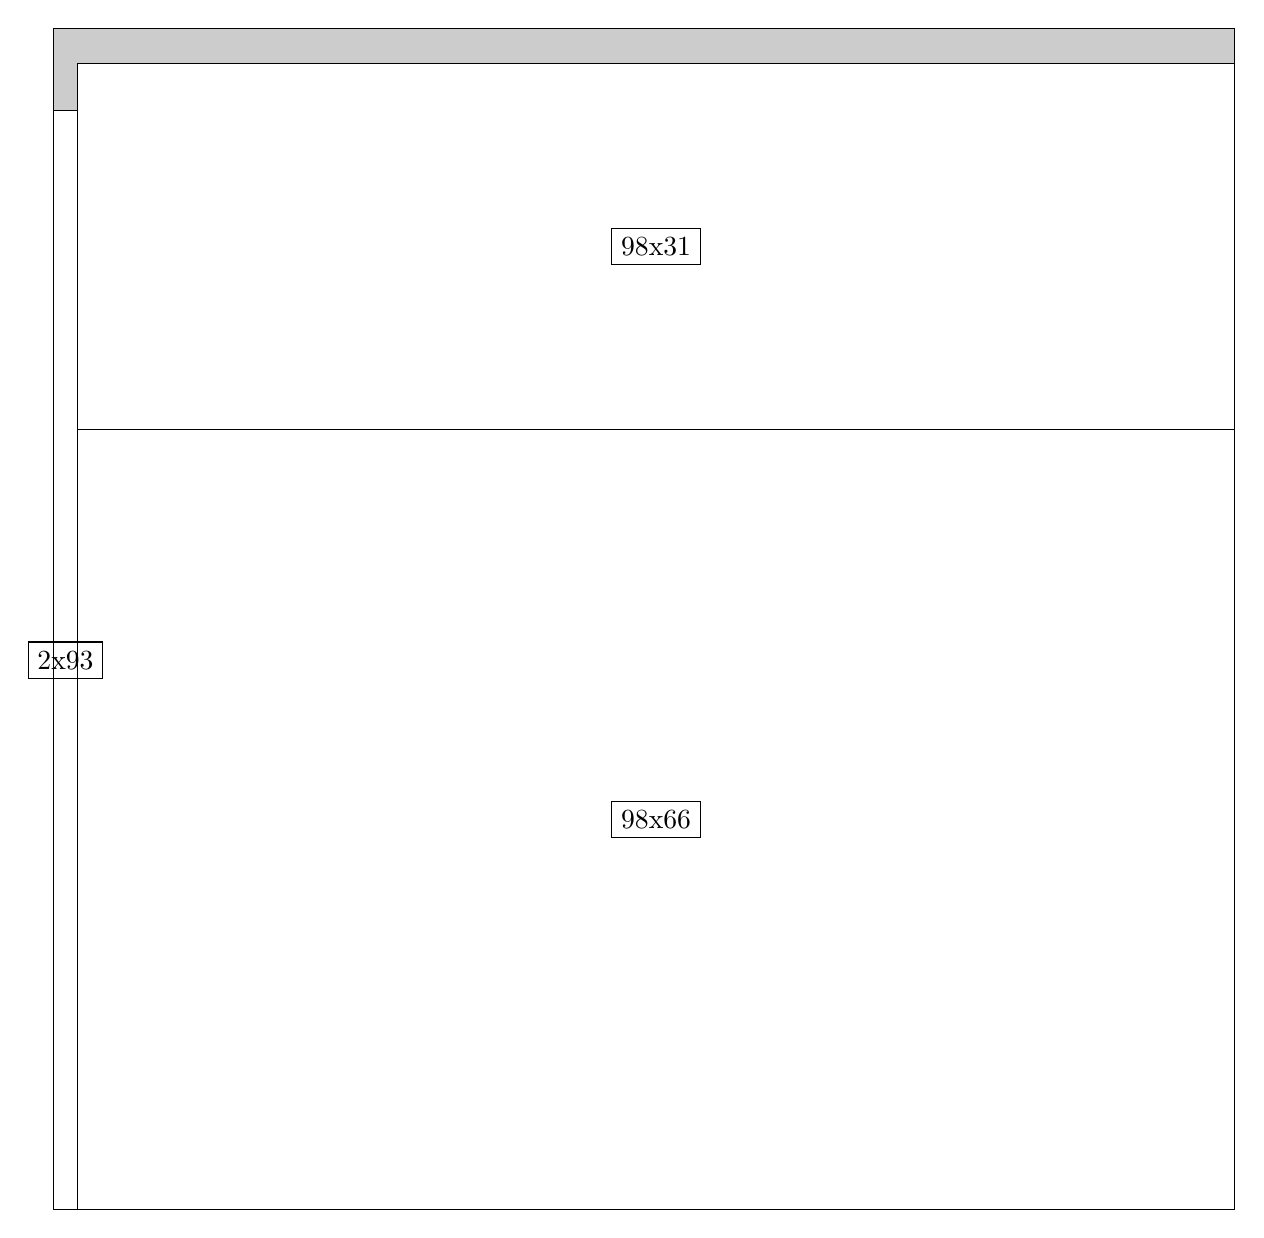
\begin{tikzpicture}[shorten >=1pt,scale=1.0,every node/.style={scale=1.0},->]
\tikzstyle{vertex}=[circle,fill=black!25,minimum size=14pt,inner sep=0pt]
\filldraw[fill=gray!40!white, draw=black] (0,0) rectangle (15.0,15.0);
\foreach \name/\x/\y/\w/\h in {98x66/0.3/0.0/14.7/9.9,98x31/0.3/9.9/14.7/4.6499999999999995,2x93/0.0/0.0/0.3/13.95}
\filldraw[fill=white!40!white, draw=black] (\x,\y) rectangle node[draw] (\name) {\name} ++(\w,\h);
\end{tikzpicture}


w =98 , h =66 , x =2 , y =0 , v =6468
\par
w =98 , h =31 , x =2 , y =66 , v =3038
\par
w =2 , h =93 , x =0 , y =0 , v =186
\par
\newpage


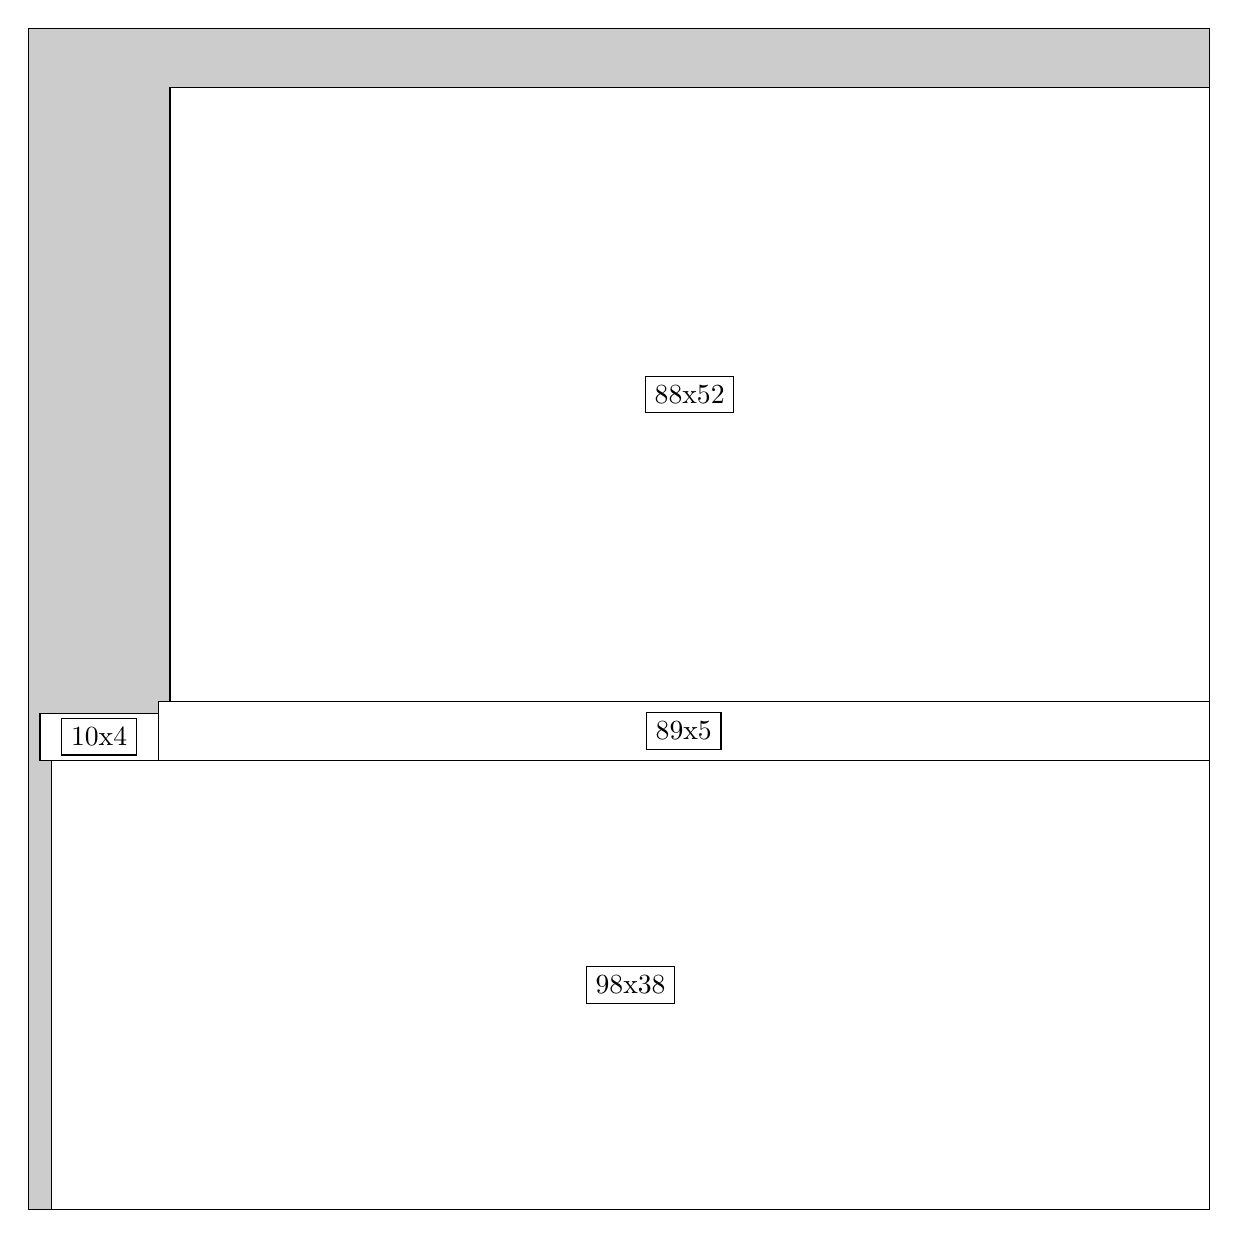
\begin{tikzpicture}[shorten >=1pt,scale=1.0,every node/.style={scale=1.0},->]
\tikzstyle{vertex}=[circle,fill=black!25,minimum size=14pt,inner sep=0pt]
\filldraw[fill=gray!40!white, draw=black] (0,0) rectangle (15.0,15.0);
\foreach \name/\x/\y/\w/\h in {98x38/0.3/0.0/14.7/5.7,89x5/1.65/5.7/13.35/0.75,10x4/0.15/5.7/1.5/0.6,88x52/1.7999999999999998/6.45/13.2/7.8}
\filldraw[fill=white!40!white, draw=black] (\x,\y) rectangle node[draw] (\name) {\name} ++(\w,\h);
\end{tikzpicture}


w =98 , h =38 , x =2 , y =0 , v =3724
\par
w =89 , h =5 , x =11 , y =38 , v =445
\par
w =10 , h =4 , x =1 , y =38 , v =40
\par
w =88 , h =52 , x =12 , y =43 , v =4576
\par
\newpage


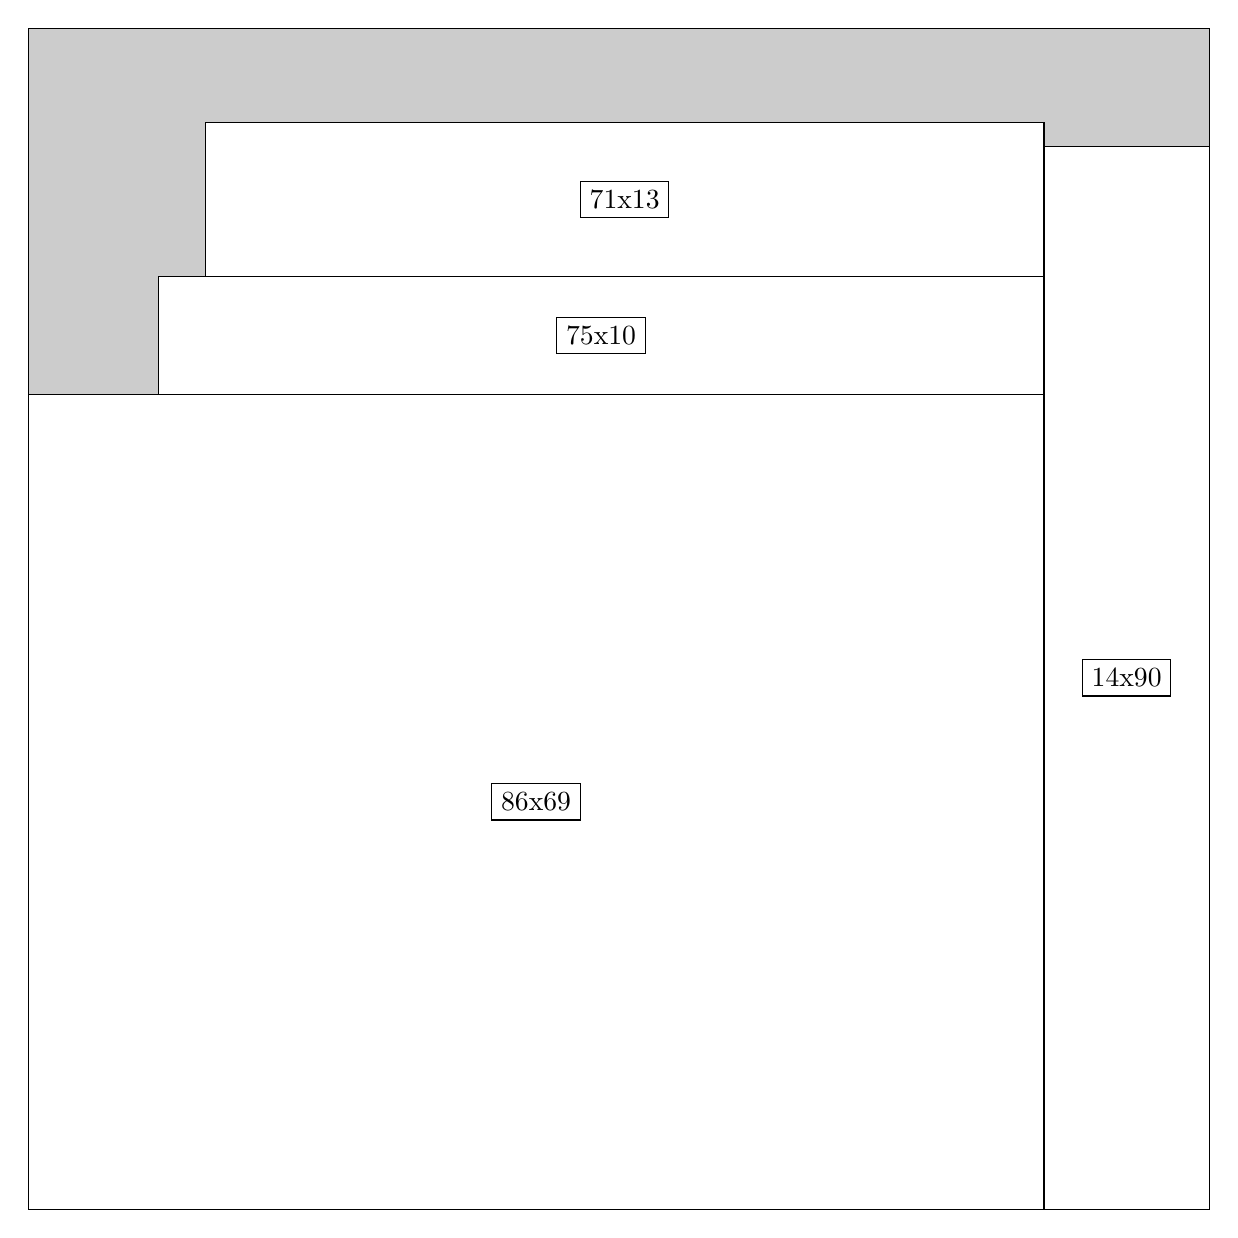
\begin{tikzpicture}[shorten >=1pt,scale=1.0,every node/.style={scale=1.0},->]
\tikzstyle{vertex}=[circle,fill=black!25,minimum size=14pt,inner sep=0pt]
\filldraw[fill=gray!40!white, draw=black] (0,0) rectangle (15.0,15.0);
\foreach \name/\x/\y/\w/\h in {14x90/12.9/0.0/2.1/13.5,86x69/0.0/0.0/12.9/10.35,75x10/1.65/10.35/11.25/1.5,71x13/2.25/11.85/10.65/1.95}
\filldraw[fill=white!40!white, draw=black] (\x,\y) rectangle node[draw] (\name) {\name} ++(\w,\h);
\end{tikzpicture}


w =14 , h =90 , x =86 , y =0 , v =1260
\par
w =86 , h =69 , x =0 , y =0 , v =5934
\par
w =75 , h =10 , x =11 , y =69 , v =750
\par
w =71 , h =13 , x =15 , y =79 , v =923
\par
\newpage


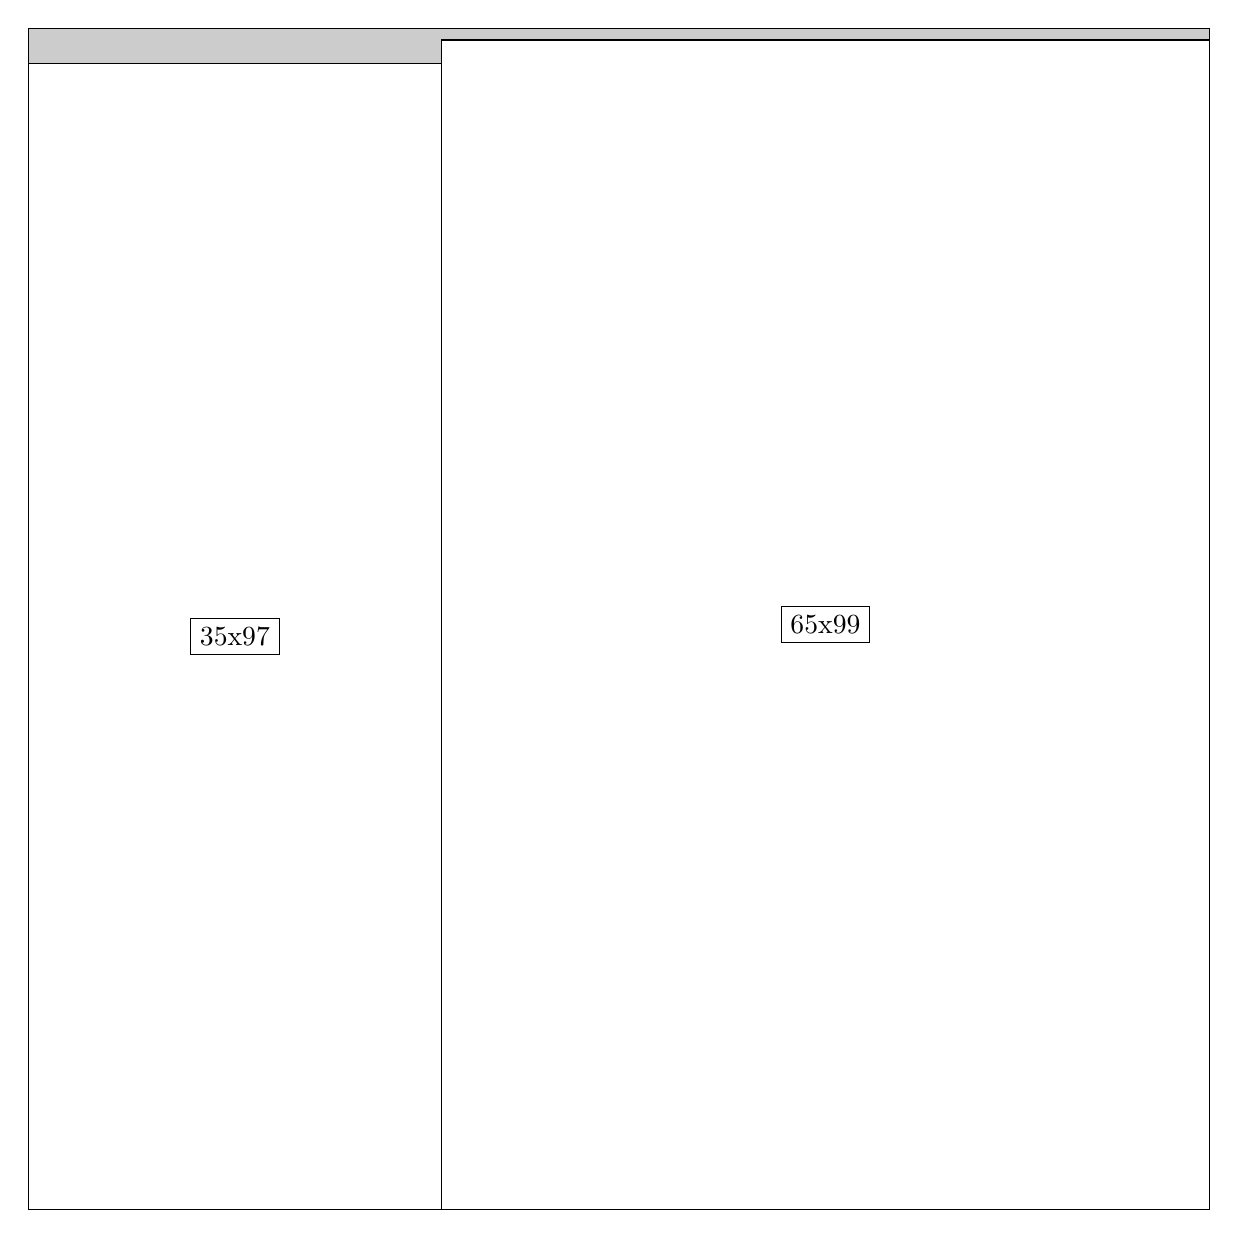
\begin{tikzpicture}[shorten >=1pt,scale=1.0,every node/.style={scale=1.0},->]
\tikzstyle{vertex}=[circle,fill=black!25,minimum size=14pt,inner sep=0pt]
\filldraw[fill=gray!40!white, draw=black] (0,0) rectangle (15.0,15.0);
\foreach \name/\x/\y/\w/\h in {65x99/5.25/0.0/9.75/14.85,35x97/0.0/0.0/5.25/14.549999999999999}
\filldraw[fill=white!40!white, draw=black] (\x,\y) rectangle node[draw] (\name) {\name} ++(\w,\h);
\end{tikzpicture}


w =65 , h =99 , x =35 , y =0 , v =6435
\par
w =35 , h =97 , x =0 , y =0 , v =3395
\par
\newpage


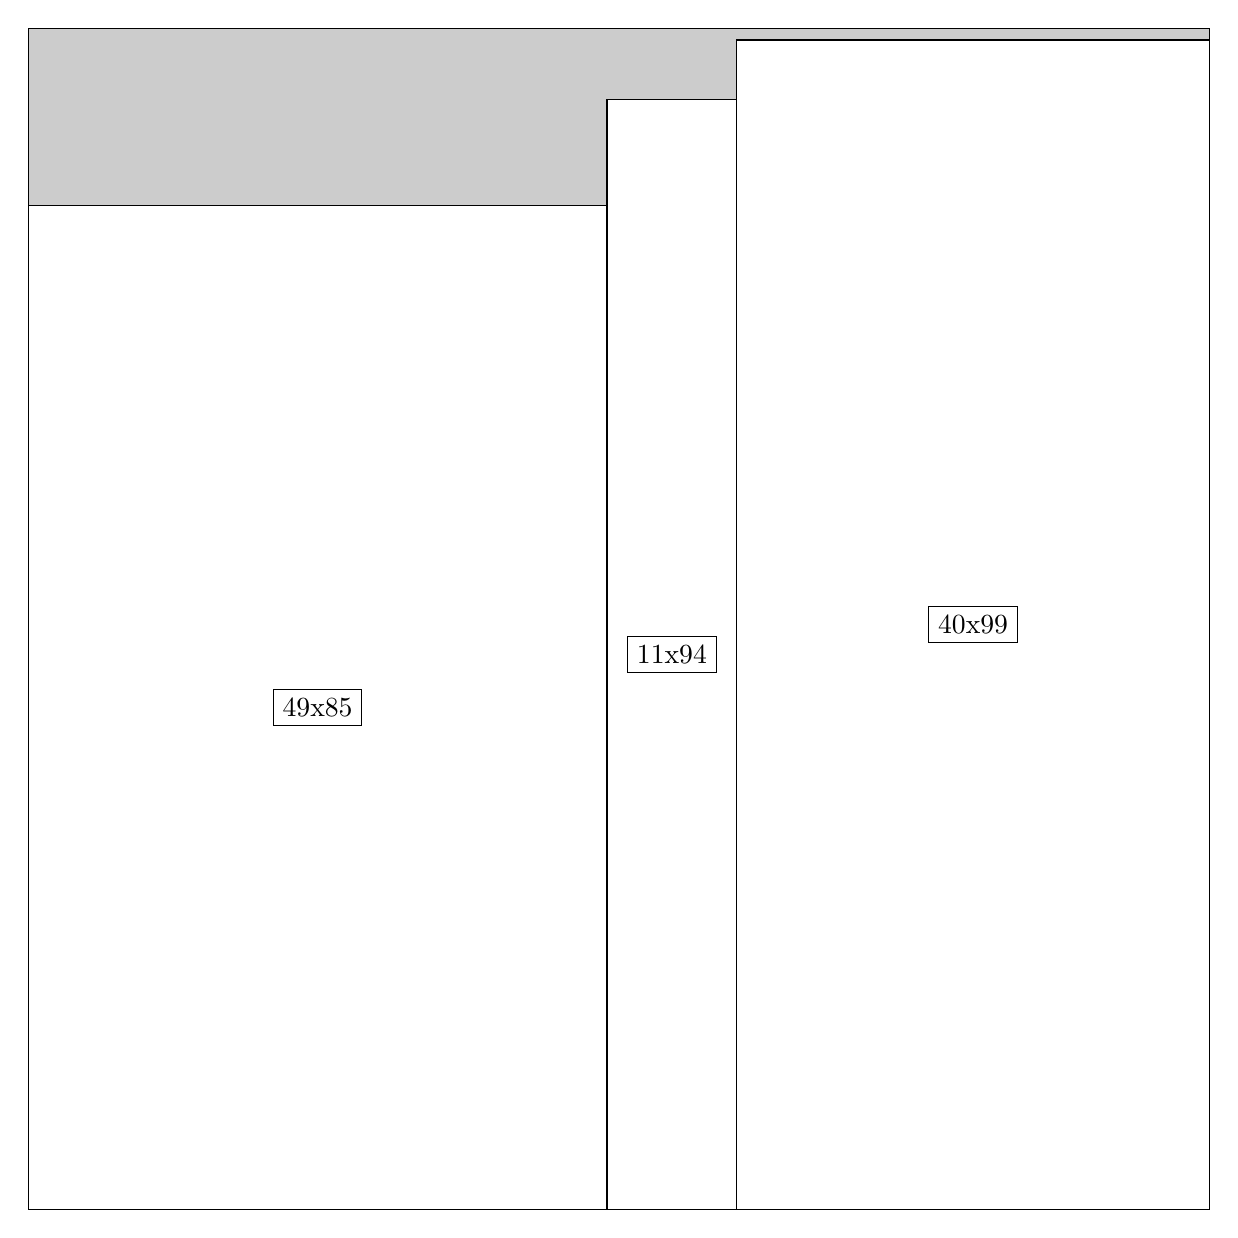
\begin{tikzpicture}[shorten >=1pt,scale=1.0,every node/.style={scale=1.0},->]
\tikzstyle{vertex}=[circle,fill=black!25,minimum size=14pt,inner sep=0pt]
\filldraw[fill=gray!40!white, draw=black] (0,0) rectangle (15.0,15.0);
\foreach \name/\x/\y/\w/\h in {40x99/9.0/0.0/6.0/14.85,11x94/7.35/0.0/1.65/14.1,49x85/0.0/0.0/7.35/12.75}
\filldraw[fill=white!40!white, draw=black] (\x,\y) rectangle node[draw] (\name) {\name} ++(\w,\h);
\end{tikzpicture}


w =40 , h =99 , x =60 , y =0 , v =3960
\par
w =11 , h =94 , x =49 , y =0 , v =1034
\par
w =49 , h =85 , x =0 , y =0 , v =4165
\par
\newpage


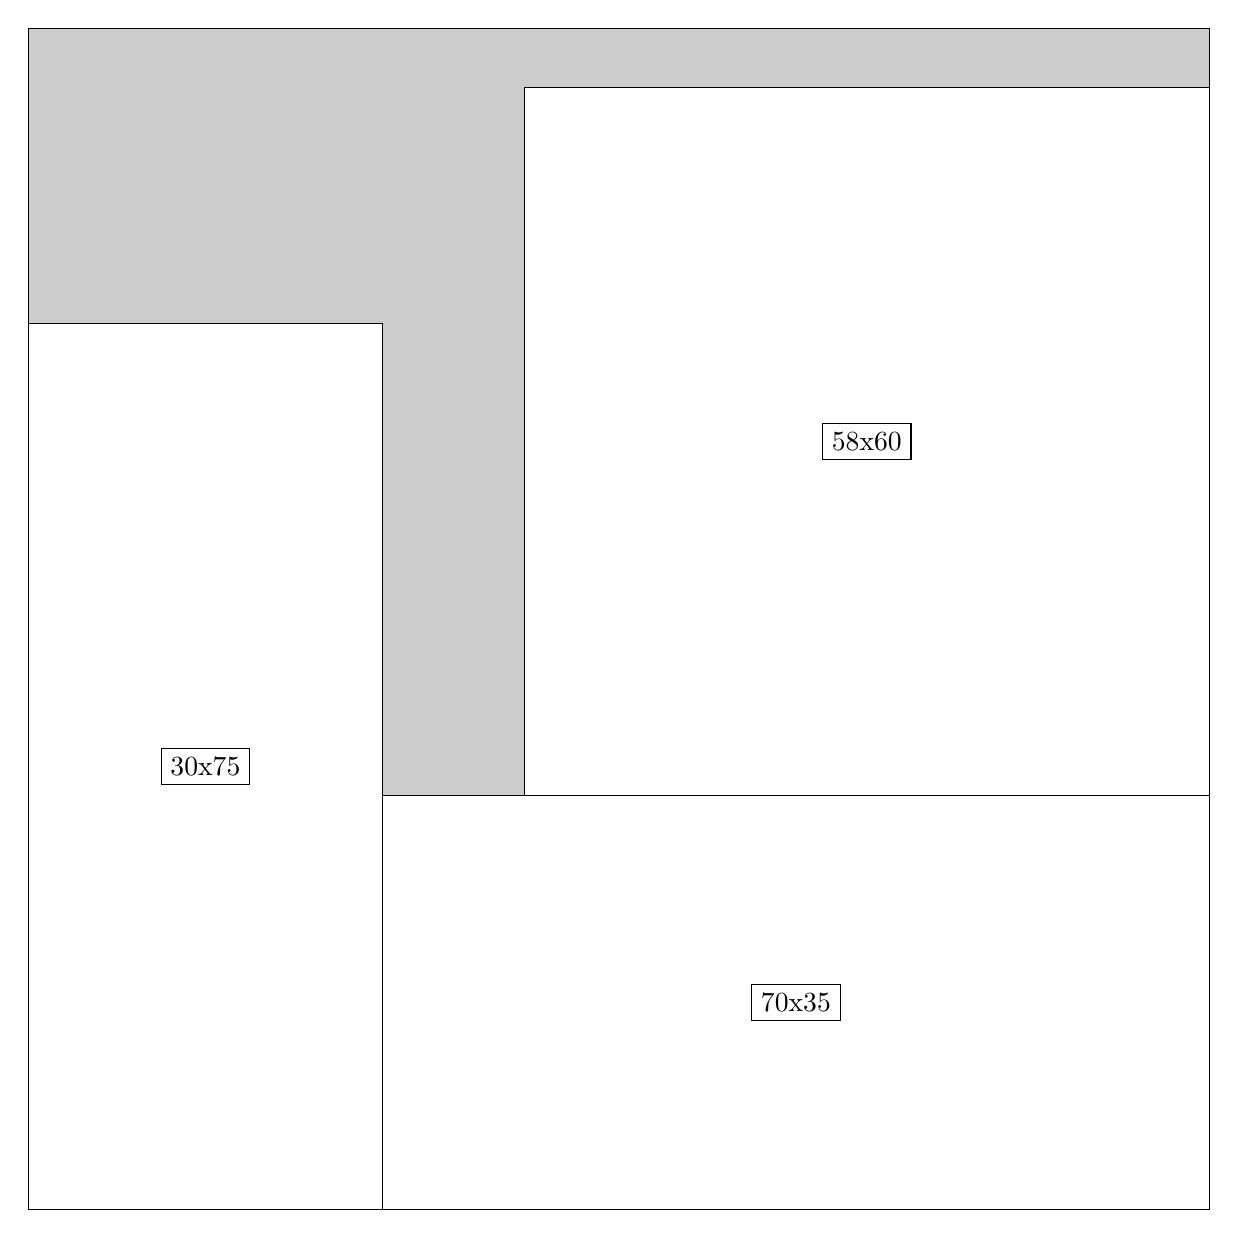
\begin{tikzpicture}[shorten >=1pt,scale=1.0,every node/.style={scale=1.0},->]
\tikzstyle{vertex}=[circle,fill=black!25,minimum size=14pt,inner sep=0pt]
\filldraw[fill=gray!40!white, draw=black] (0,0) rectangle (15.0,15.0);
\foreach \name/\x/\y/\w/\h in {70x35/4.5/0.0/10.5/5.25,58x60/6.3/5.25/8.7/9.0,30x75/0.0/0.0/4.5/11.25}
\filldraw[fill=white!40!white, draw=black] (\x,\y) rectangle node[draw] (\name) {\name} ++(\w,\h);
\end{tikzpicture}


w =70 , h =35 , x =30 , y =0 , v =2450
\par
w =58 , h =60 , x =42 , y =35 , v =3480
\par
w =30 , h =75 , x =0 , y =0 , v =2250
\par
\newpage


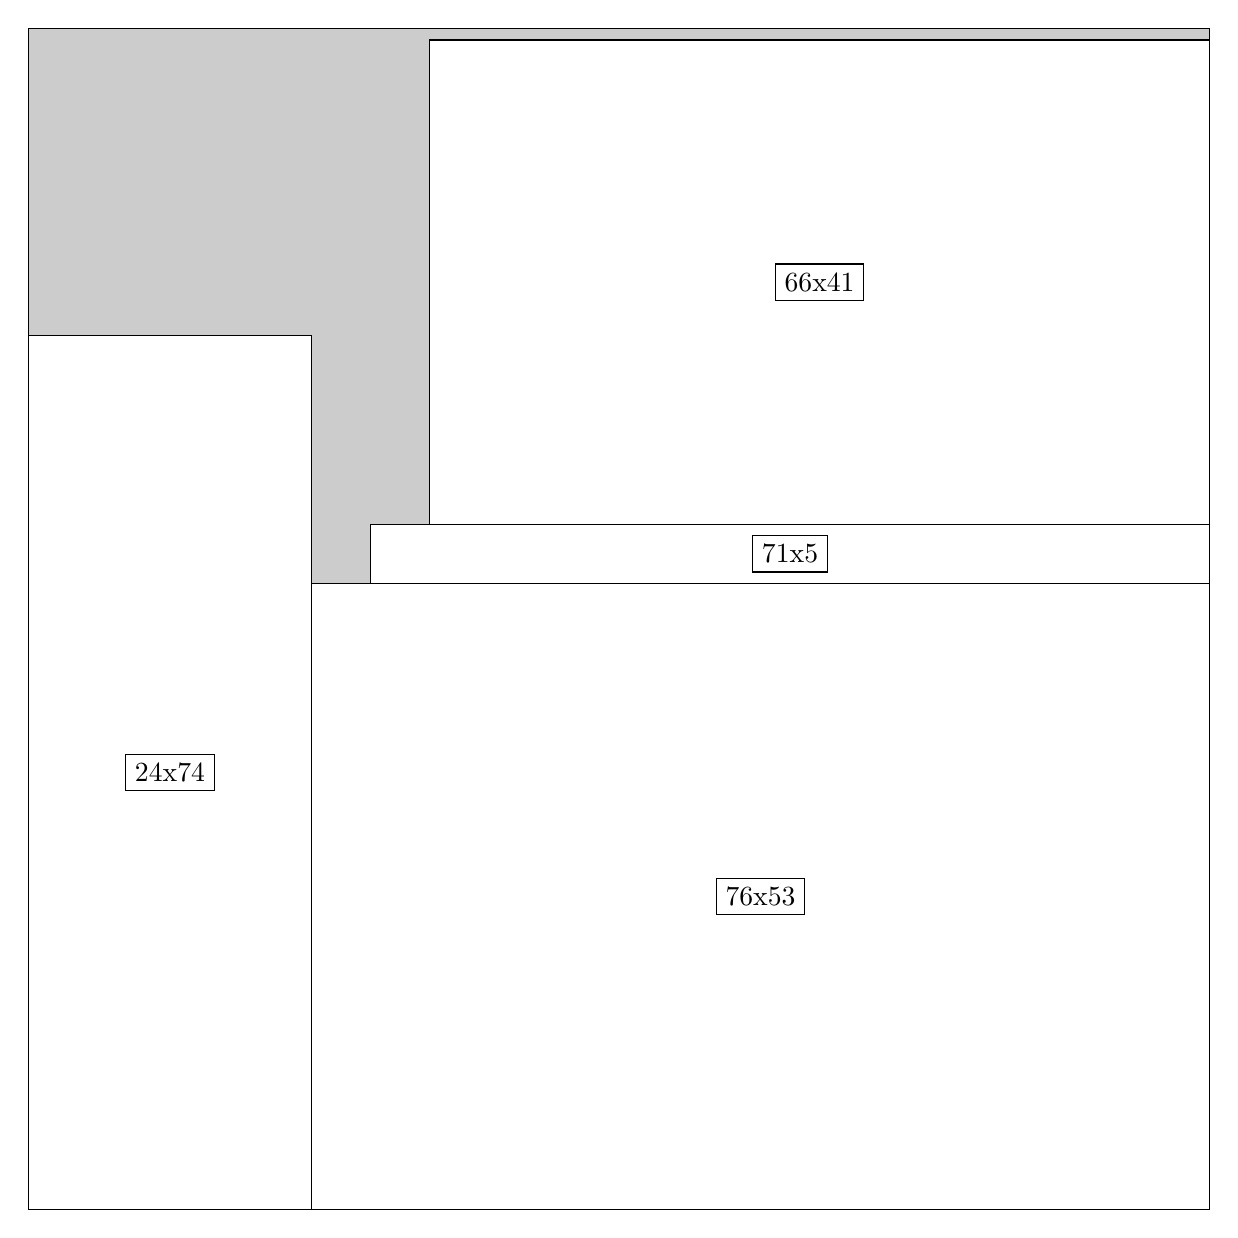
\begin{tikzpicture}[shorten >=1pt,scale=1.0,every node/.style={scale=1.0},->]
\tikzstyle{vertex}=[circle,fill=black!25,minimum size=14pt,inner sep=0pt]
\filldraw[fill=gray!40!white, draw=black] (0,0) rectangle (15.0,15.0);
\foreach \name/\x/\y/\w/\h in {76x53/3.5999999999999996/0.0/11.4/7.949999999999999,71x5/4.35/7.949999999999999/10.65/0.75,66x41/5.1/8.7/9.9/6.1499999999999995,24x74/0.0/0.0/3.5999999999999996/11.1}
\filldraw[fill=white!40!white, draw=black] (\x,\y) rectangle node[draw] (\name) {\name} ++(\w,\h);
\end{tikzpicture}


w =76 , h =53 , x =24 , y =0 , v =4028
\par
w =71 , h =5 , x =29 , y =53 , v =355
\par
w =66 , h =41 , x =34 , y =58 , v =2706
\par
w =24 , h =74 , x =0 , y =0 , v =1776
\par
\newpage


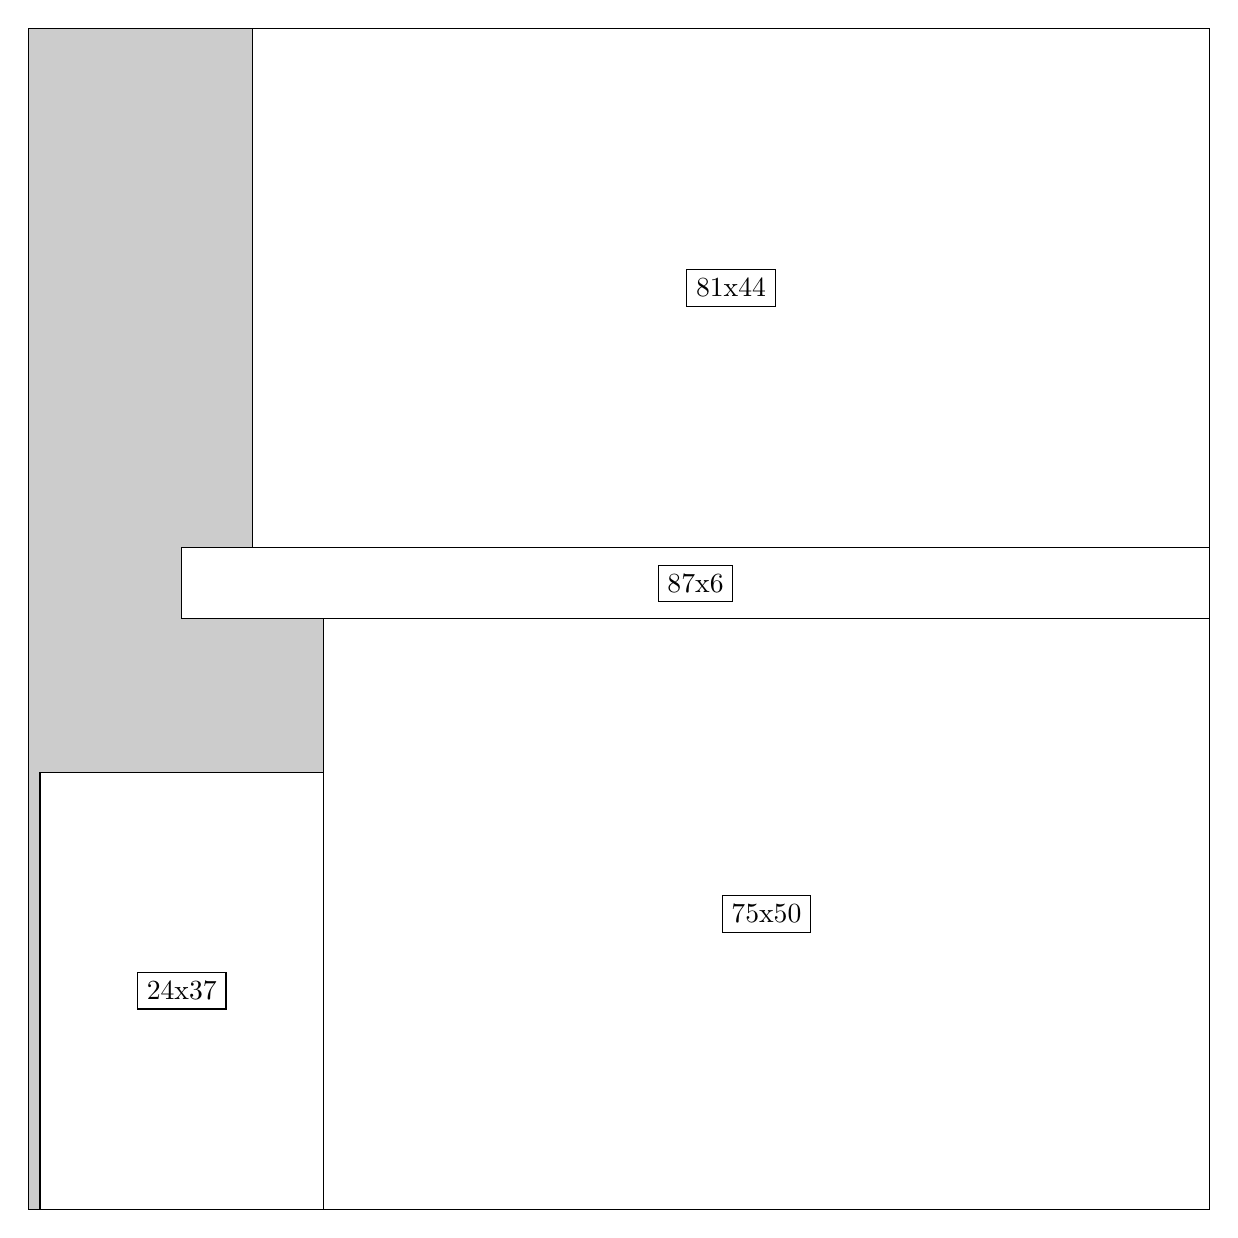
\begin{tikzpicture}[shorten >=1pt,scale=1.0,every node/.style={scale=1.0},->]
\tikzstyle{vertex}=[circle,fill=black!25,minimum size=14pt,inner sep=0pt]
\filldraw[fill=gray!40!white, draw=black] (0,0) rectangle (15.0,15.0);
\foreach \name/\x/\y/\w/\h in {75x50/3.75/0.0/11.25/7.5,24x37/0.15/0.0/3.5999999999999996/5.55,87x6/1.95/7.5/13.049999999999999/0.8999999999999999,81x44/2.85/8.4/12.15/6.6}
\filldraw[fill=white!40!white, draw=black] (\x,\y) rectangle node[draw] (\name) {\name} ++(\w,\h);
\end{tikzpicture}


w =75 , h =50 , x =25 , y =0 , v =3750
\par
w =24 , h =37 , x =1 , y =0 , v =888
\par
w =87 , h =6 , x =13 , y =50 , v =522
\par
w =81 , h =44 , x =19 , y =56 , v =3564
\par
\newpage


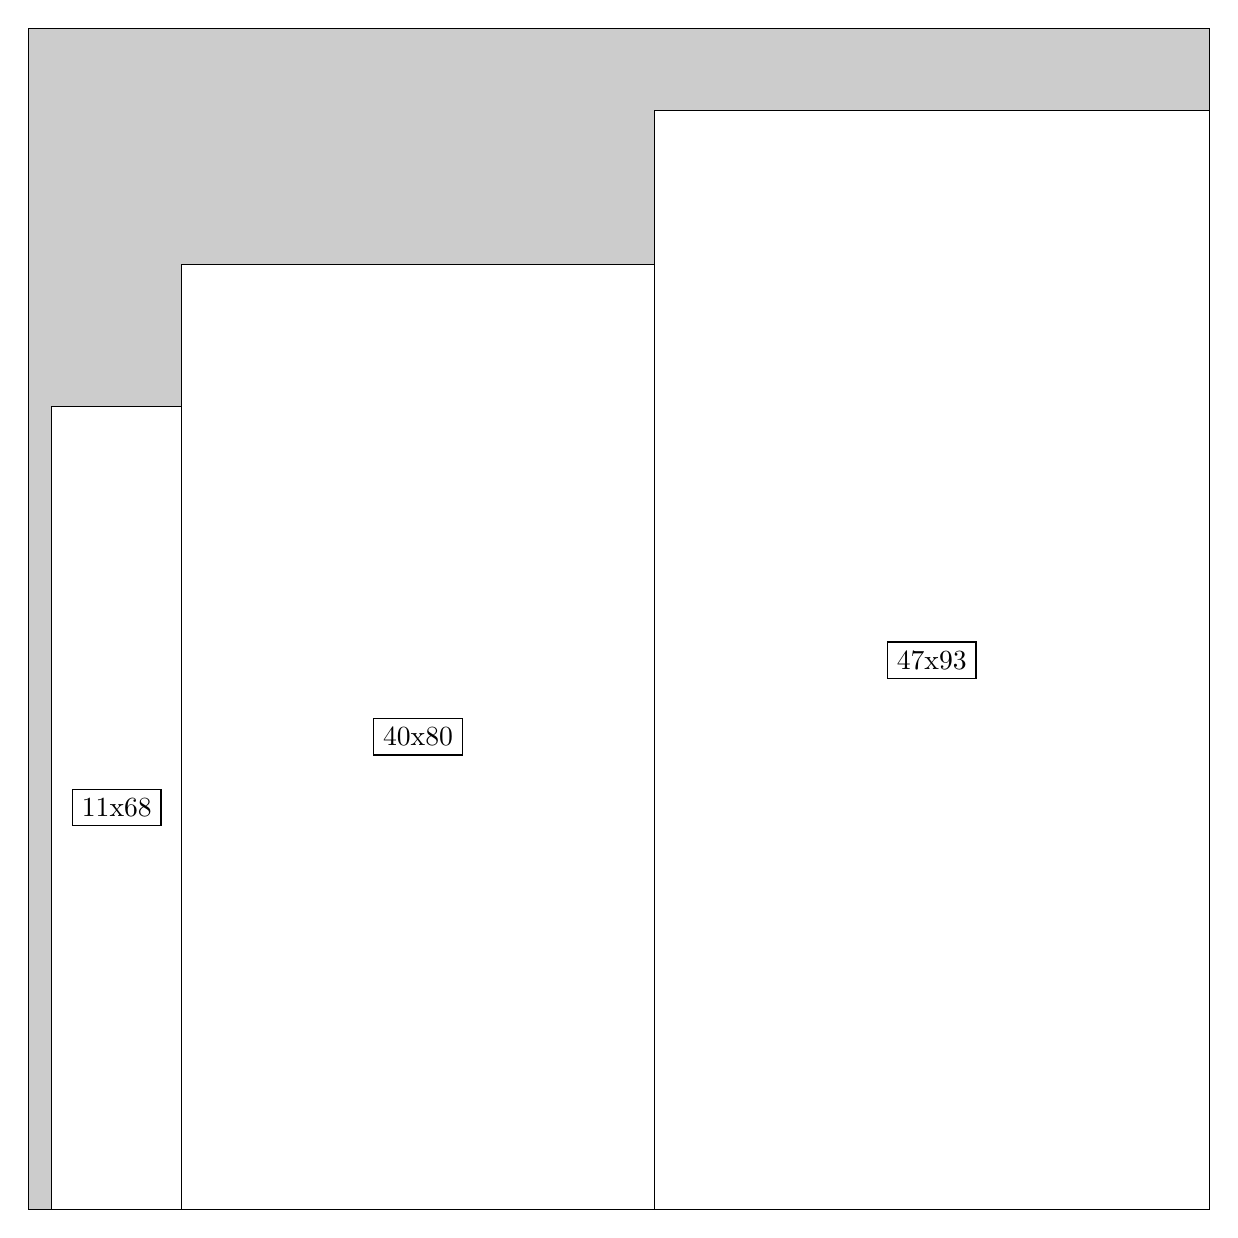
\begin{tikzpicture}[shorten >=1pt,scale=1.0,every node/.style={scale=1.0},->]
\tikzstyle{vertex}=[circle,fill=black!25,minimum size=14pt,inner sep=0pt]
\filldraw[fill=gray!40!white, draw=black] (0,0) rectangle (15.0,15.0);
\foreach \name/\x/\y/\w/\h in {47x93/7.949999999999999/0.0/7.05/13.95,40x80/1.95/0.0/6.0/12.0,11x68/0.3/0.0/1.65/10.2}
\filldraw[fill=white!40!white, draw=black] (\x,\y) rectangle node[draw] (\name) {\name} ++(\w,\h);
\end{tikzpicture}


w =47 , h =93 , x =53 , y =0 , v =4371
\par
w =40 , h =80 , x =13 , y =0 , v =3200
\par
w =11 , h =68 , x =2 , y =0 , v =748
\par
\newpage


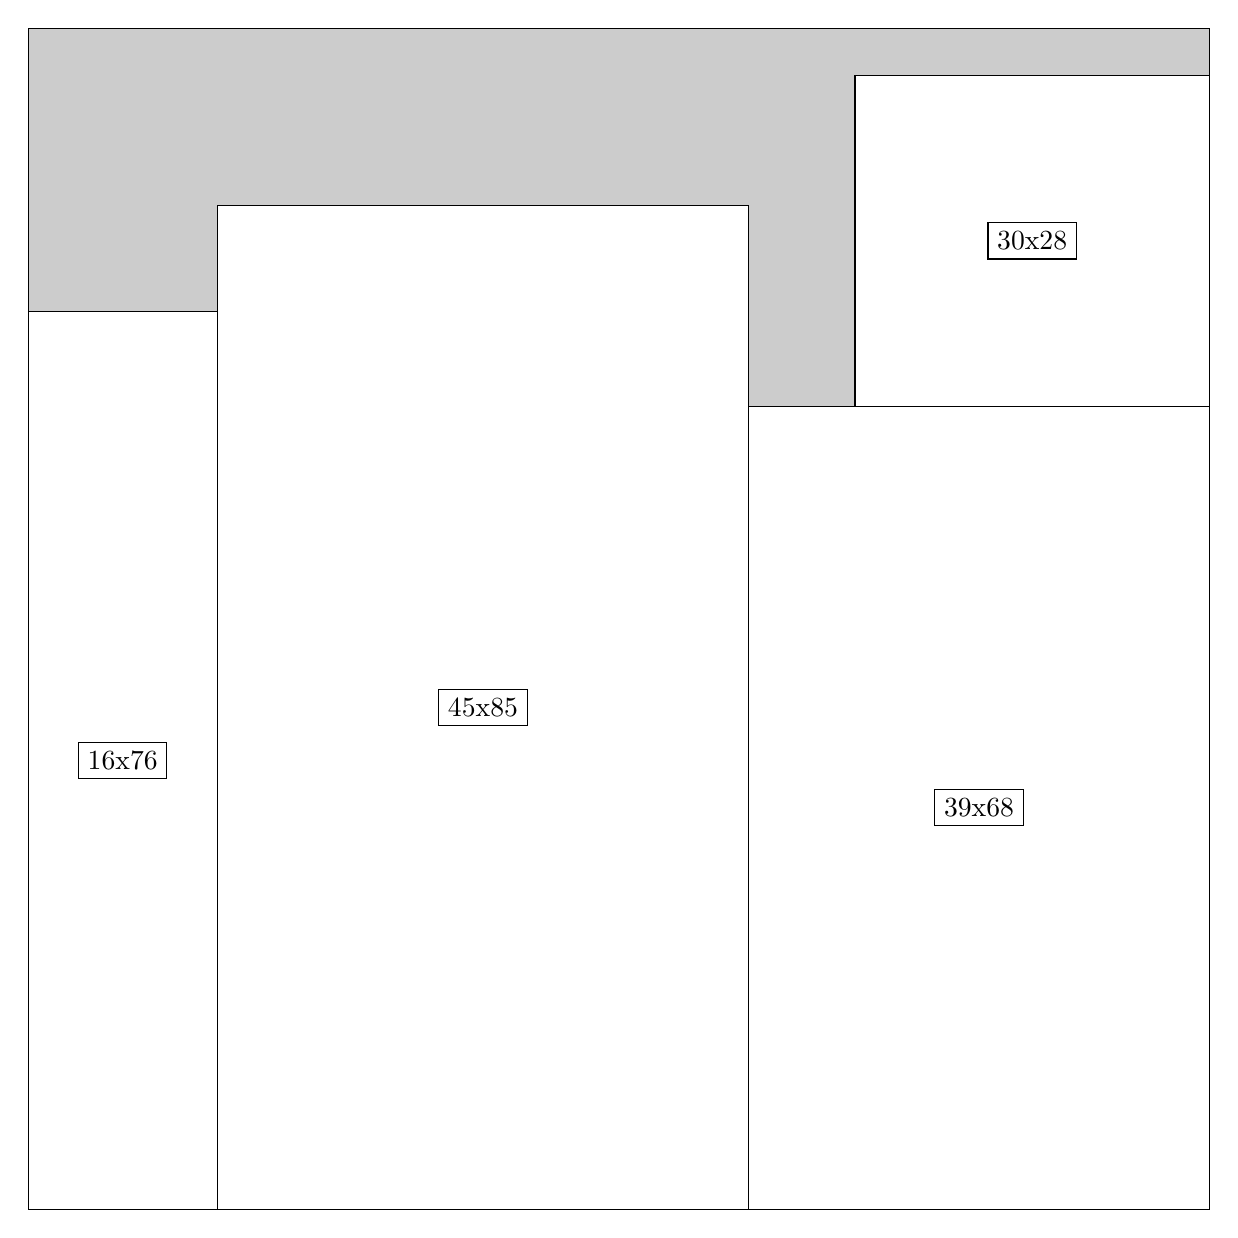
\begin{tikzpicture}[shorten >=1pt,scale=1.0,every node/.style={scale=1.0},->]
\tikzstyle{vertex}=[circle,fill=black!25,minimum size=14pt,inner sep=0pt]
\filldraw[fill=gray!40!white, draw=black] (0,0) rectangle (15.0,15.0);
\foreach \name/\x/\y/\w/\h in {39x68/9.15/0.0/5.85/10.2,30x28/10.5/10.2/4.5/4.2,45x85/2.4/0.0/6.75/12.75,16x76/0.0/0.0/2.4/11.4}
\filldraw[fill=white!40!white, draw=black] (\x,\y) rectangle node[draw] (\name) {\name} ++(\w,\h);
\end{tikzpicture}


w =39 , h =68 , x =61 , y =0 , v =2652
\par
w =30 , h =28 , x =70 , y =68 , v =840
\par
w =45 , h =85 , x =16 , y =0 , v =3825
\par
w =16 , h =76 , x =0 , y =0 , v =1216
\par
\newpage


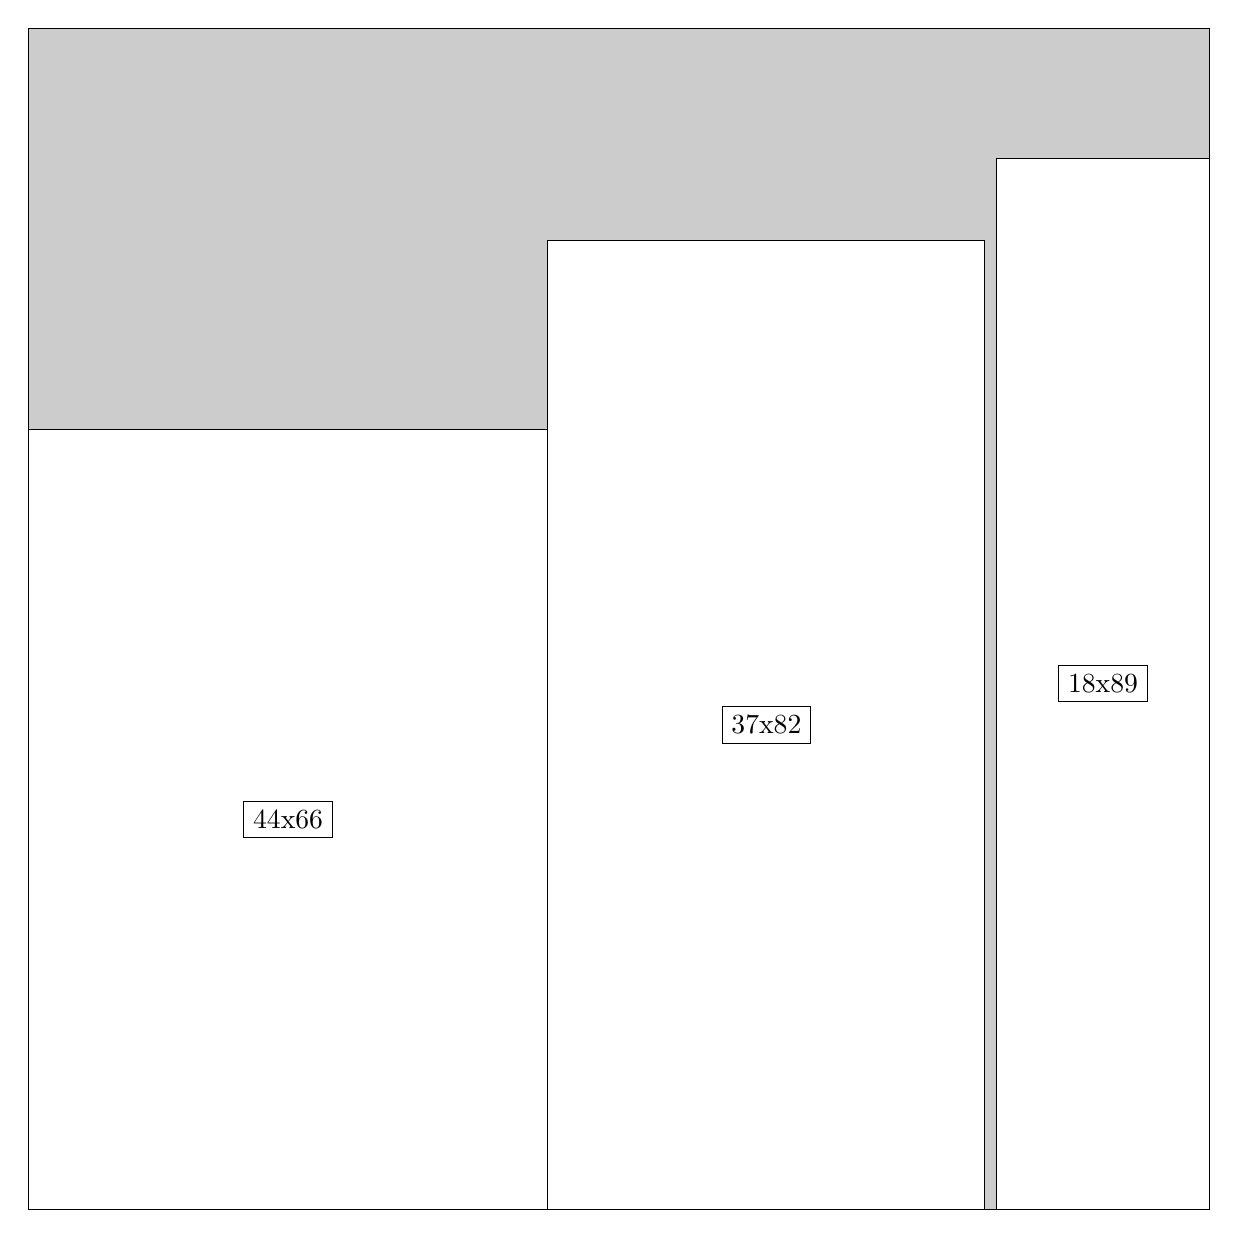
\begin{tikzpicture}[shorten >=1pt,scale=1.0,every node/.style={scale=1.0},->]
\tikzstyle{vertex}=[circle,fill=black!25,minimum size=14pt,inner sep=0pt]
\filldraw[fill=gray!40!white, draw=black] (0,0) rectangle (15.0,15.0);
\foreach \name/\x/\y/\w/\h in {18x89/12.299999999999999/0.0/2.6999999999999997/13.35,37x82/6.6/0.0/5.55/12.299999999999999,44x66/0.0/0.0/6.6/9.9}
\filldraw[fill=white!40!white, draw=black] (\x,\y) rectangle node[draw] (\name) {\name} ++(\w,\h);
\end{tikzpicture}


w =18 , h =89 , x =82 , y =0 , v =1602
\par
w =37 , h =82 , x =44 , y =0 , v =3034
\par
w =44 , h =66 , x =0 , y =0 , v =2904
\par
\newpage


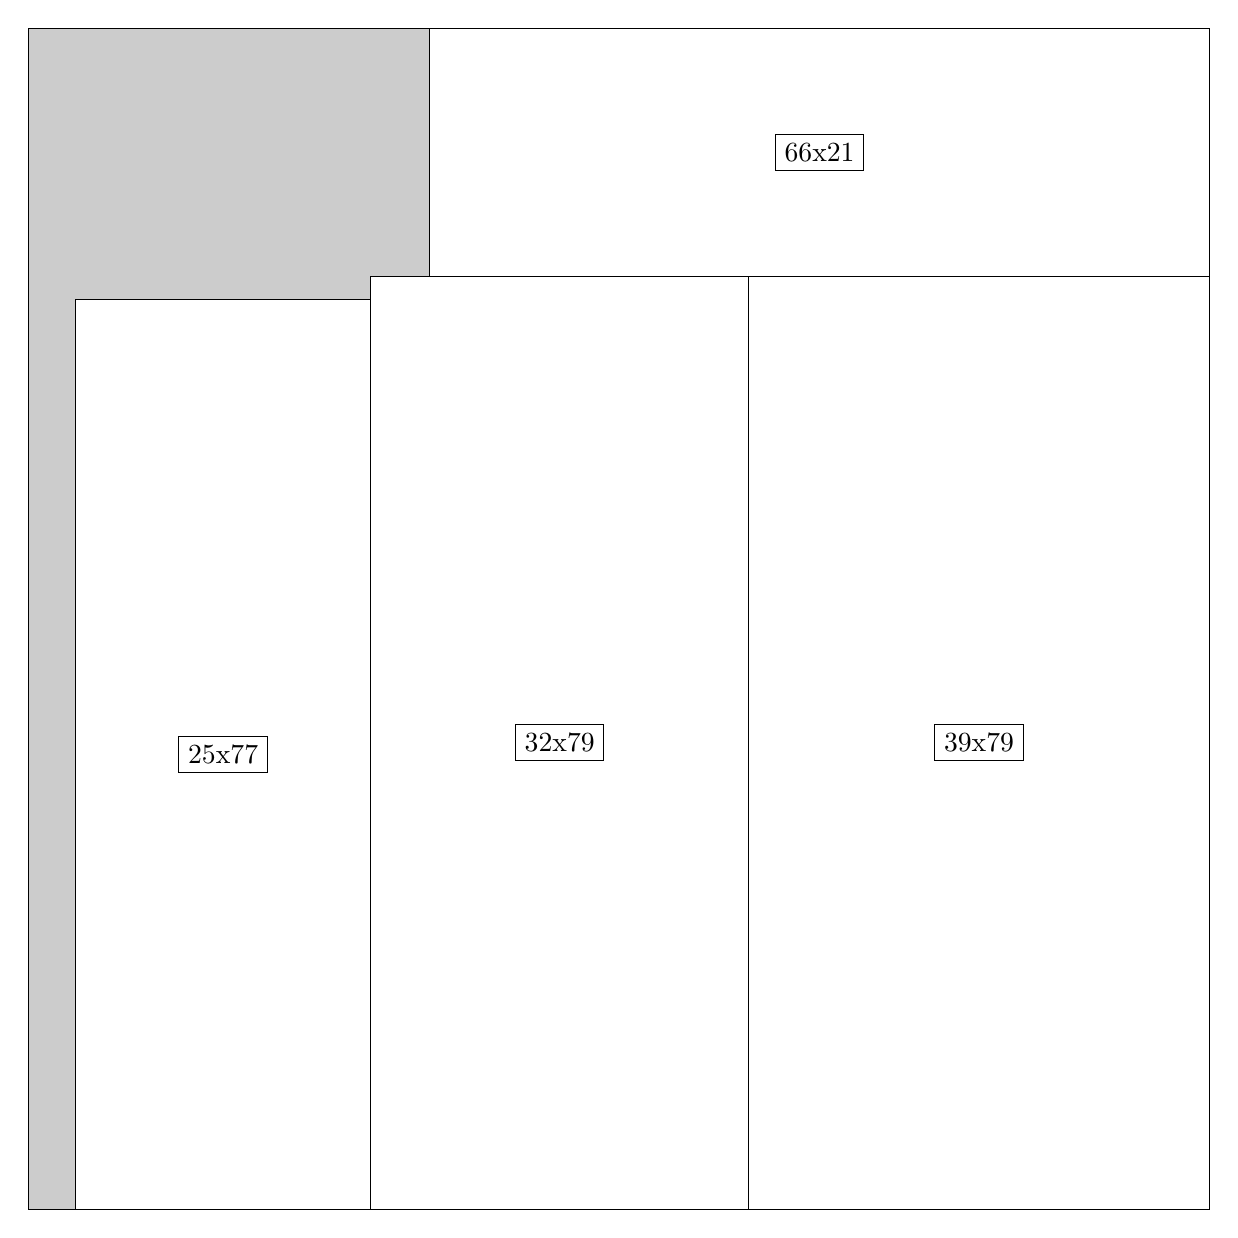
\begin{tikzpicture}[shorten >=1pt,scale=1.0,every node/.style={scale=1.0},->]
\tikzstyle{vertex}=[circle,fill=black!25,minimum size=14pt,inner sep=0pt]
\filldraw[fill=gray!40!white, draw=black] (0,0) rectangle (15.0,15.0);
\foreach \name/\x/\y/\w/\h in {39x79/9.15/0.0/5.85/11.85,32x79/4.35/0.0/4.8/11.85,25x77/0.6/0.0/3.75/11.549999999999999,66x21/5.1/11.85/9.9/3.15}
\filldraw[fill=white!40!white, draw=black] (\x,\y) rectangle node[draw] (\name) {\name} ++(\w,\h);
\end{tikzpicture}


w =39 , h =79 , x =61 , y =0 , v =3081
\par
w =32 , h =79 , x =29 , y =0 , v =2528
\par
w =25 , h =77 , x =4 , y =0 , v =1925
\par
w =66 , h =21 , x =34 , y =79 , v =1386
\par
\newpage


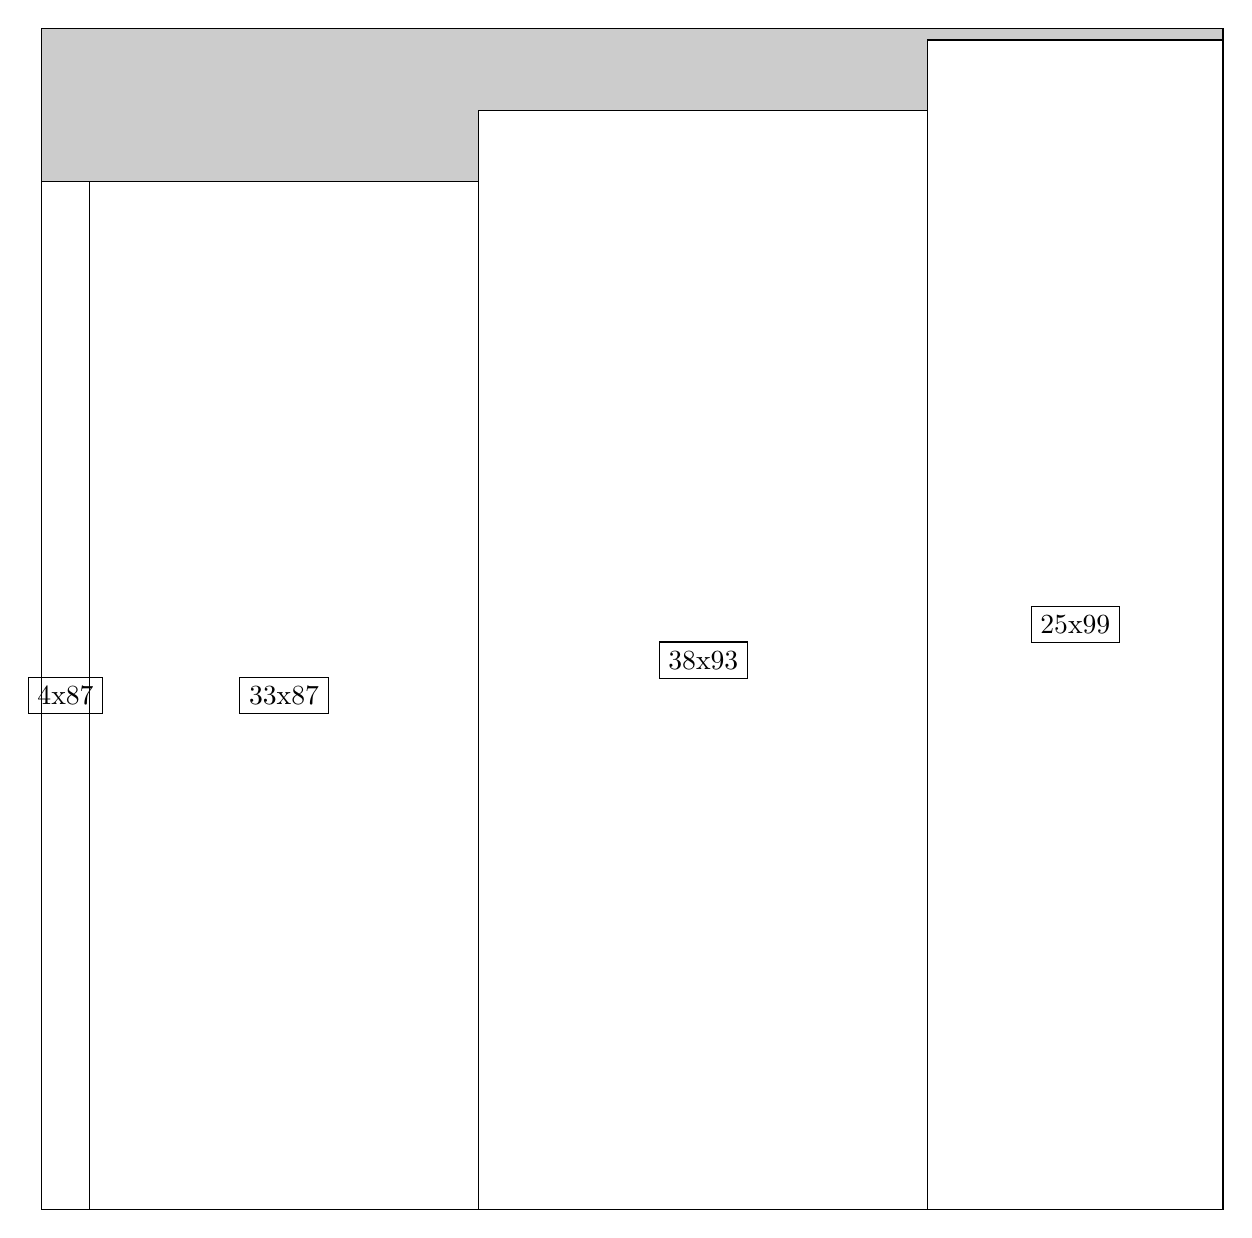
\begin{tikzpicture}[shorten >=1pt,scale=1.0,every node/.style={scale=1.0},->]
\tikzstyle{vertex}=[circle,fill=black!25,minimum size=14pt,inner sep=0pt]
\filldraw[fill=gray!40!white, draw=black] (0,0) rectangle (15.0,15.0);
\foreach \name/\x/\y/\w/\h in {25x99/11.25/0.0/3.75/14.85,38x93/5.55/0.0/5.7/13.95,33x87/0.6/0.0/4.95/13.049999999999999,4x87/0.0/0.0/0.6/13.049999999999999}
\filldraw[fill=white!40!white, draw=black] (\x,\y) rectangle node[draw] (\name) {\name} ++(\w,\h);
\end{tikzpicture}


w =25 , h =99 , x =75 , y =0 , v =2475
\par
w =38 , h =93 , x =37 , y =0 , v =3534
\par
w =33 , h =87 , x =4 , y =0 , v =2871
\par
w =4 , h =87 , x =0 , y =0 , v =348
\par
\newpage


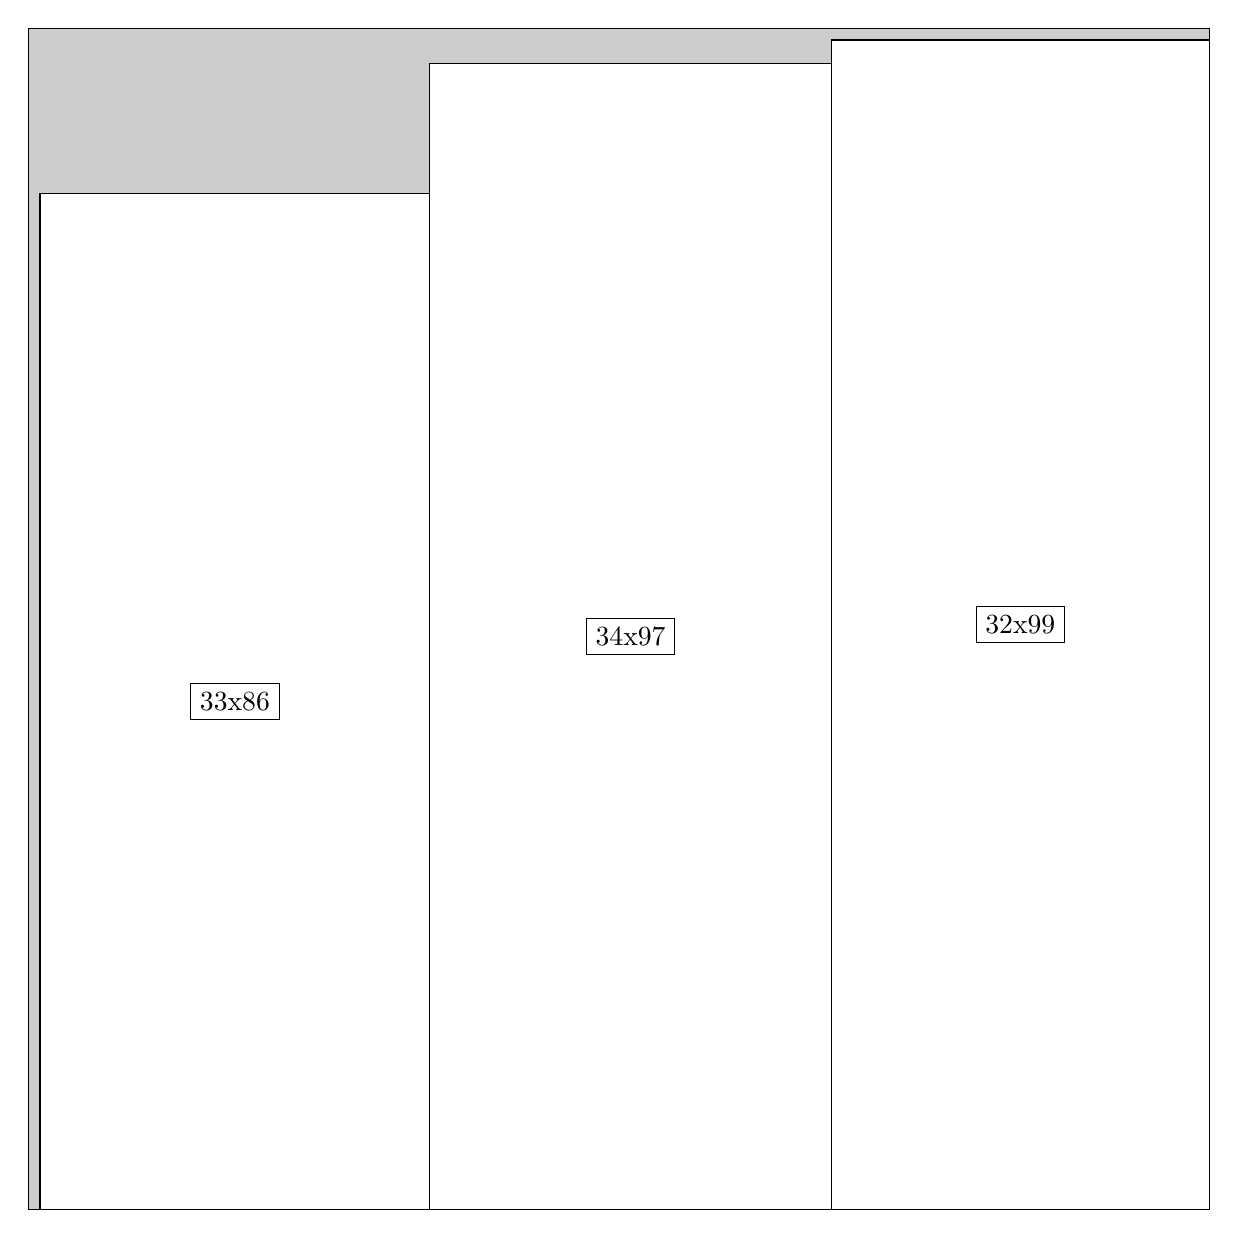
\begin{tikzpicture}[shorten >=1pt,scale=1.0,every node/.style={scale=1.0},->]
\tikzstyle{vertex}=[circle,fill=black!25,minimum size=14pt,inner sep=0pt]
\filldraw[fill=gray!40!white, draw=black] (0,0) rectangle (15.0,15.0);
\foreach \name/\x/\y/\w/\h in {32x99/10.2/0.0/4.8/14.85,34x97/5.1/0.0/5.1/14.549999999999999,33x86/0.15/0.0/4.95/12.9}
\filldraw[fill=white!40!white, draw=black] (\x,\y) rectangle node[draw] (\name) {\name} ++(\w,\h);
\end{tikzpicture}


w =32 , h =99 , x =68 , y =0 , v =3168
\par
w =34 , h =97 , x =34 , y =0 , v =3298
\par
w =33 , h =86 , x =1 , y =0 , v =2838
\par
\newpage


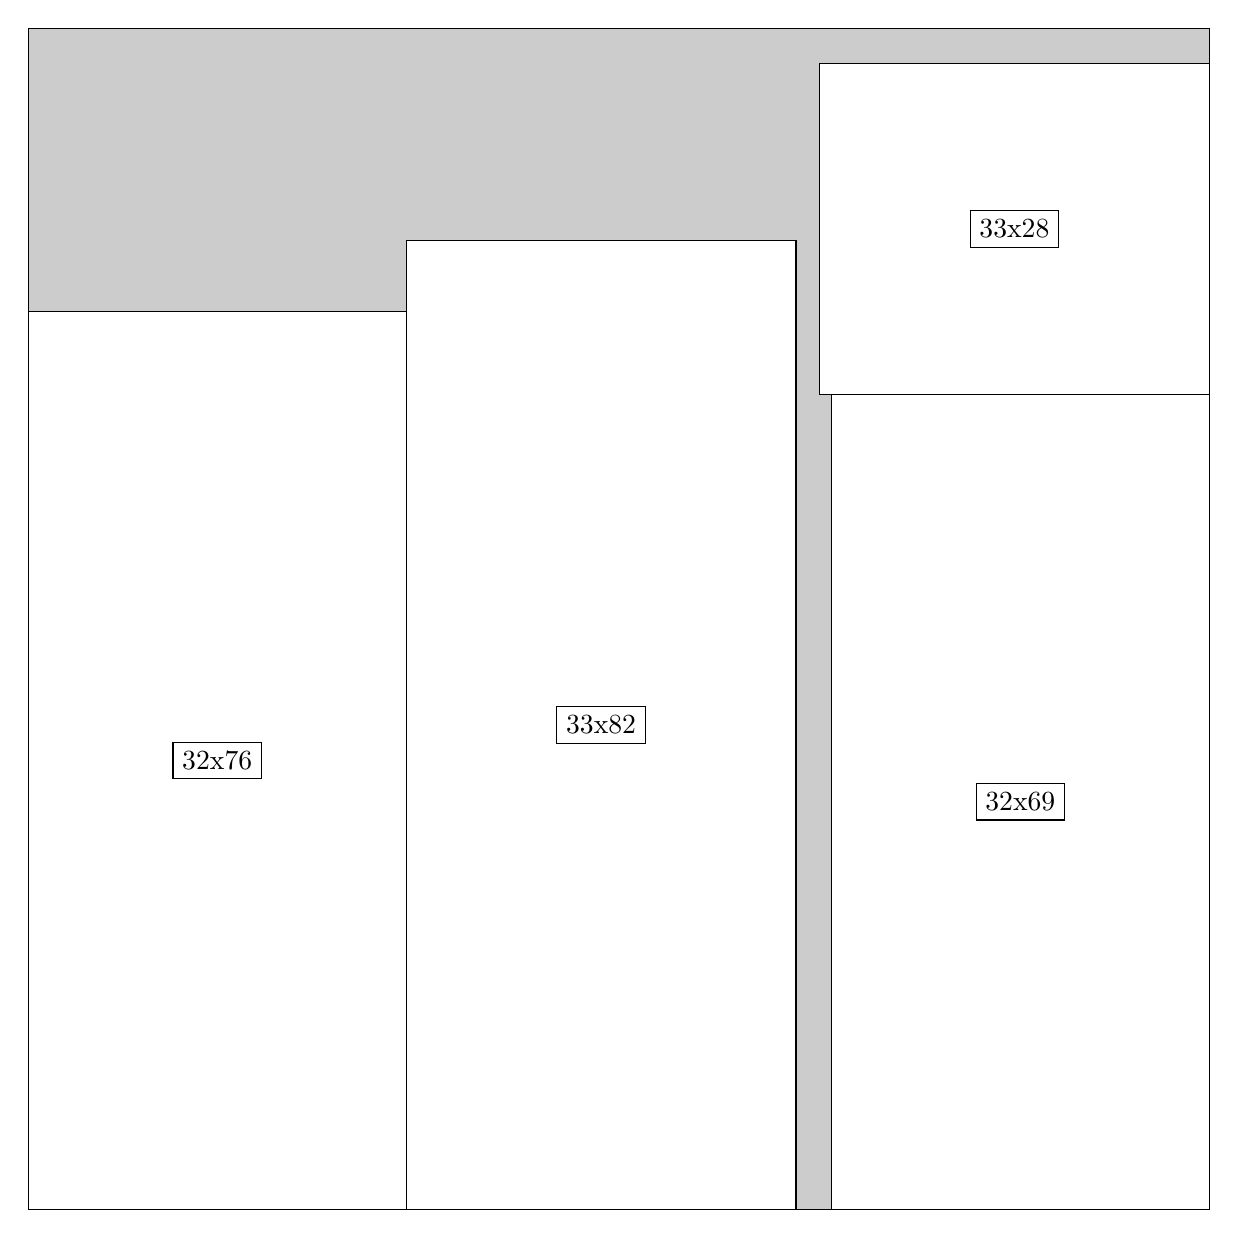
\begin{tikzpicture}[shorten >=1pt,scale=1.0,every node/.style={scale=1.0},->]
\tikzstyle{vertex}=[circle,fill=black!25,minimum size=14pt,inner sep=0pt]
\filldraw[fill=gray!40!white, draw=black] (0,0) rectangle (15.0,15.0);
\foreach \name/\x/\y/\w/\h in {32x69/10.2/0.0/4.8/10.35,33x28/10.049999999999999/10.35/4.95/4.2,33x82/4.8/0.0/4.95/12.299999999999999,32x76/0.0/0.0/4.8/11.4}
\filldraw[fill=white!40!white, draw=black] (\x,\y) rectangle node[draw] (\name) {\name} ++(\w,\h);
\end{tikzpicture}


w =32 , h =69 , x =68 , y =0 , v =2208
\par
w =33 , h =28 , x =67 , y =69 , v =924
\par
w =33 , h =82 , x =32 , y =0 , v =2706
\par
w =32 , h =76 , x =0 , y =0 , v =2432
\par
\newpage


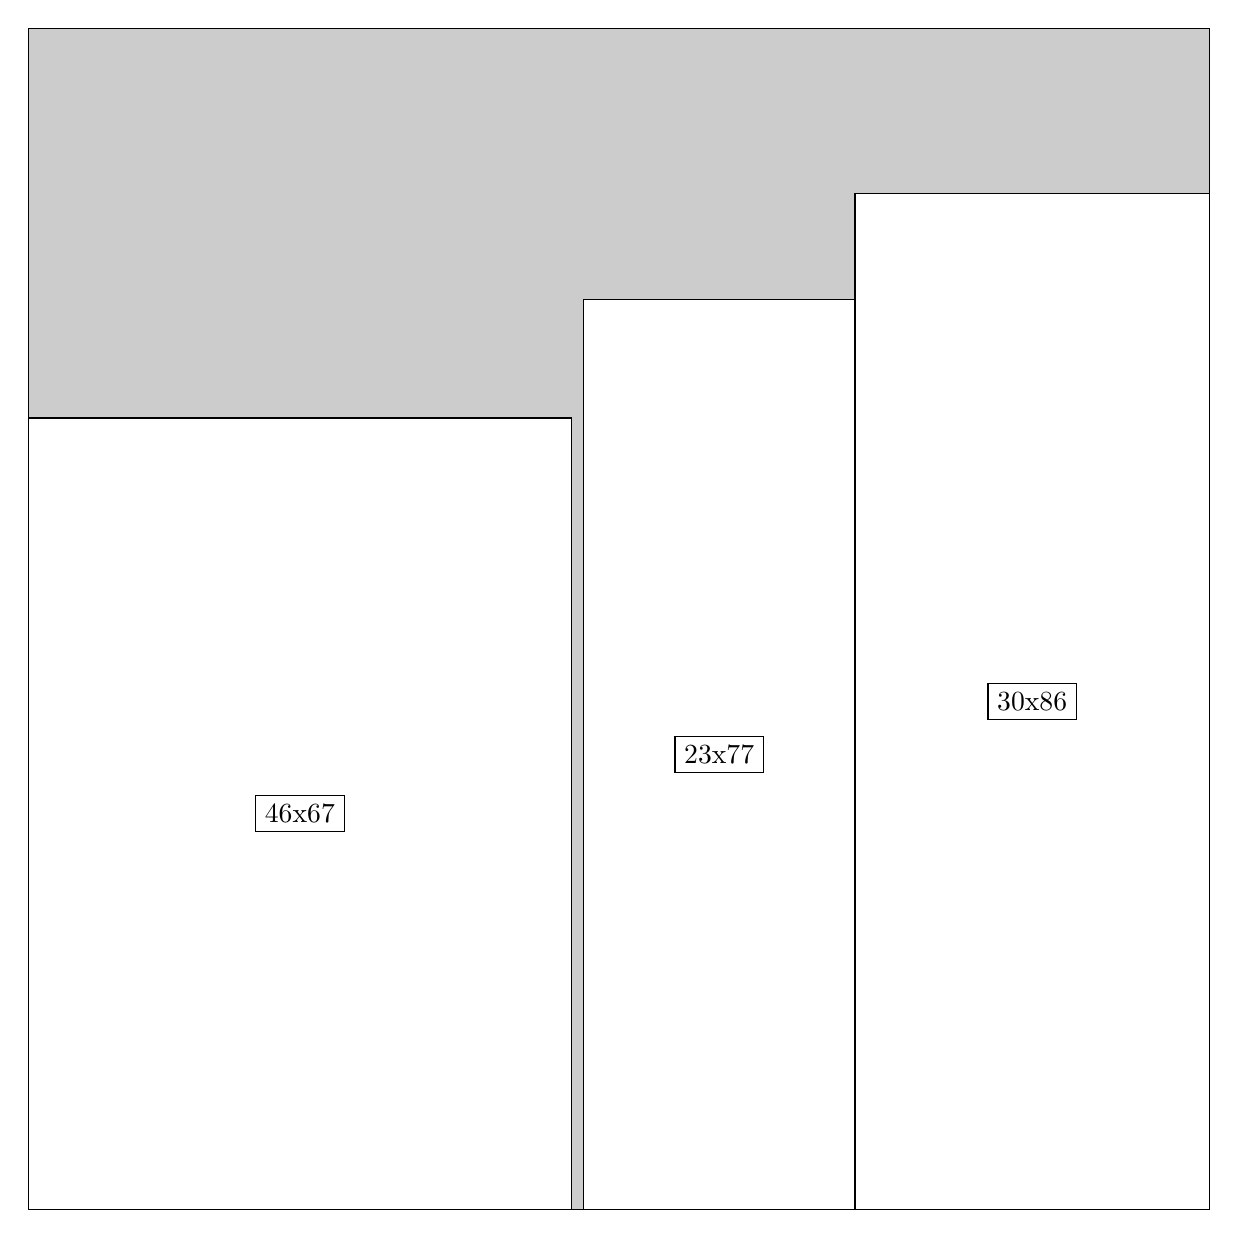
\begin{tikzpicture}[shorten >=1pt,scale=1.0,every node/.style={scale=1.0},->]
\tikzstyle{vertex}=[circle,fill=black!25,minimum size=14pt,inner sep=0pt]
\filldraw[fill=gray!40!white, draw=black] (0,0) rectangle (15.0,15.0);
\foreach \name/\x/\y/\w/\h in {30x86/10.5/0.0/4.5/12.9,23x77/7.05/0.0/3.4499999999999997/11.549999999999999,46x67/0.0/0.0/6.8999999999999995/10.049999999999999}
\filldraw[fill=white!40!white, draw=black] (\x,\y) rectangle node[draw] (\name) {\name} ++(\w,\h);
\end{tikzpicture}


w =30 , h =86 , x =70 , y =0 , v =2580
\par
w =23 , h =77 , x =47 , y =0 , v =1771
\par
w =46 , h =67 , x =0 , y =0 , v =3082
\par
\newpage


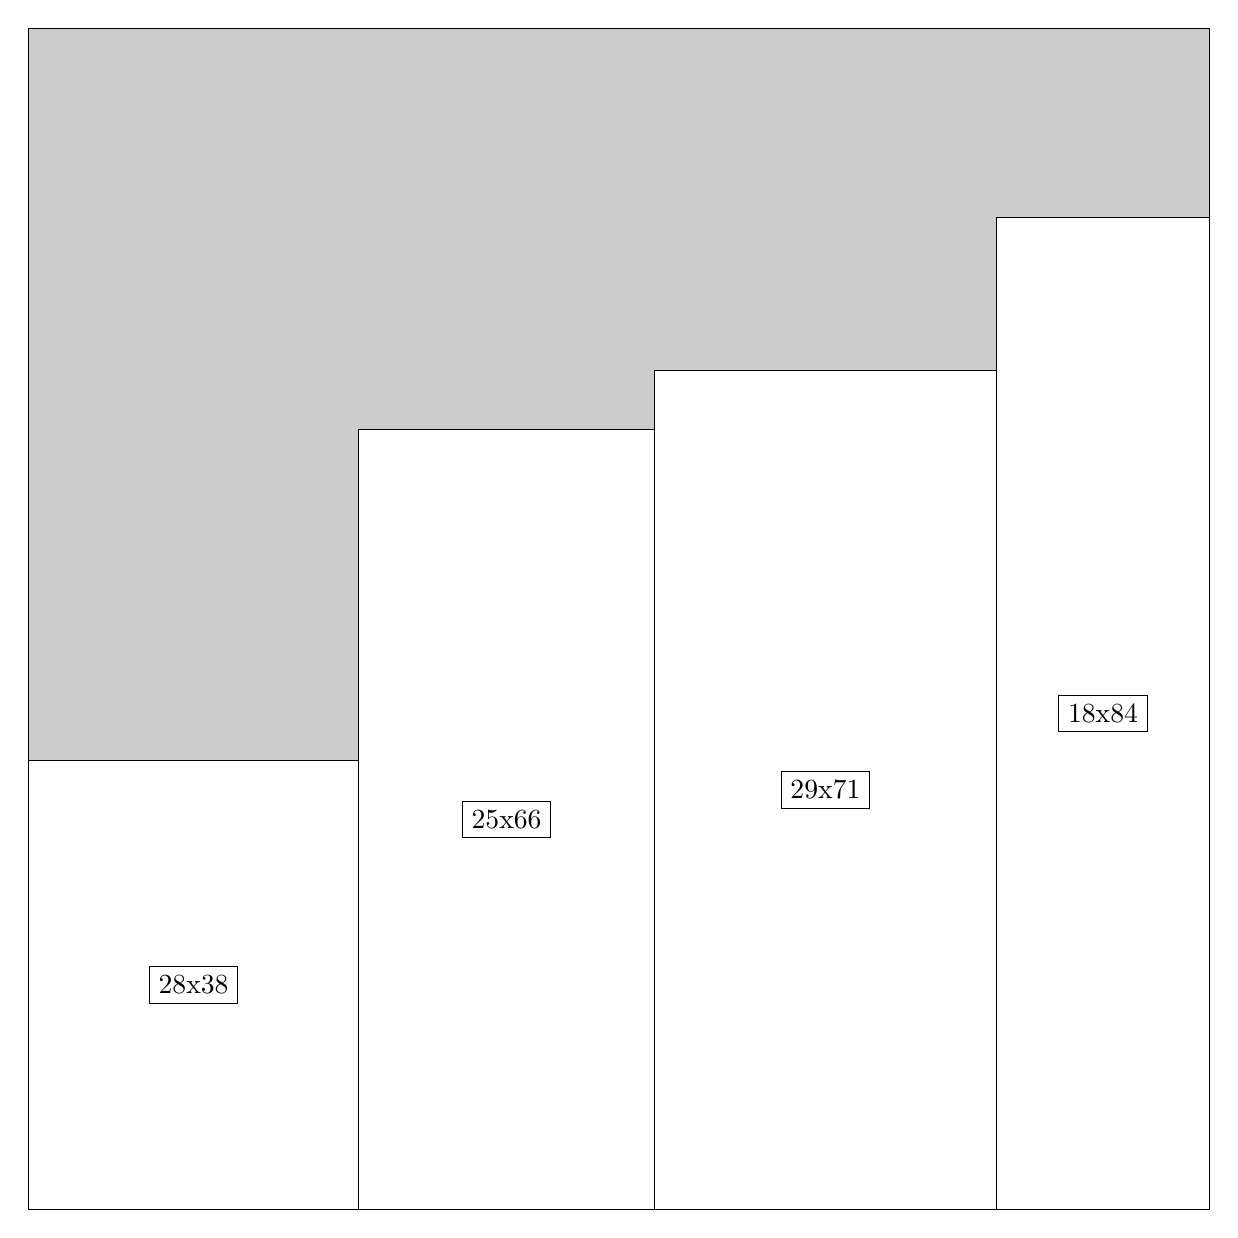
\begin{tikzpicture}[shorten >=1pt,scale=1.0,every node/.style={scale=1.0},->]
\tikzstyle{vertex}=[circle,fill=black!25,minimum size=14pt,inner sep=0pt]
\filldraw[fill=gray!40!white, draw=black] (0,0) rectangle (15.0,15.0);
\foreach \name/\x/\y/\w/\h in {18x84/12.299999999999999/0.0/2.6999999999999997/12.6,29x71/7.949999999999999/0.0/4.35/10.65,25x66/4.2/0.0/3.75/9.9,28x38/0.0/0.0/4.2/5.7}
\filldraw[fill=white!40!white, draw=black] (\x,\y) rectangle node[draw] (\name) {\name} ++(\w,\h);
\end{tikzpicture}


w =18 , h =84 , x =82 , y =0 , v =1512
\par
w =29 , h =71 , x =53 , y =0 , v =2059
\par
w =25 , h =66 , x =28 , y =0 , v =1650
\par
w =28 , h =38 , x =0 , y =0 , v =1064
\par
\newpage


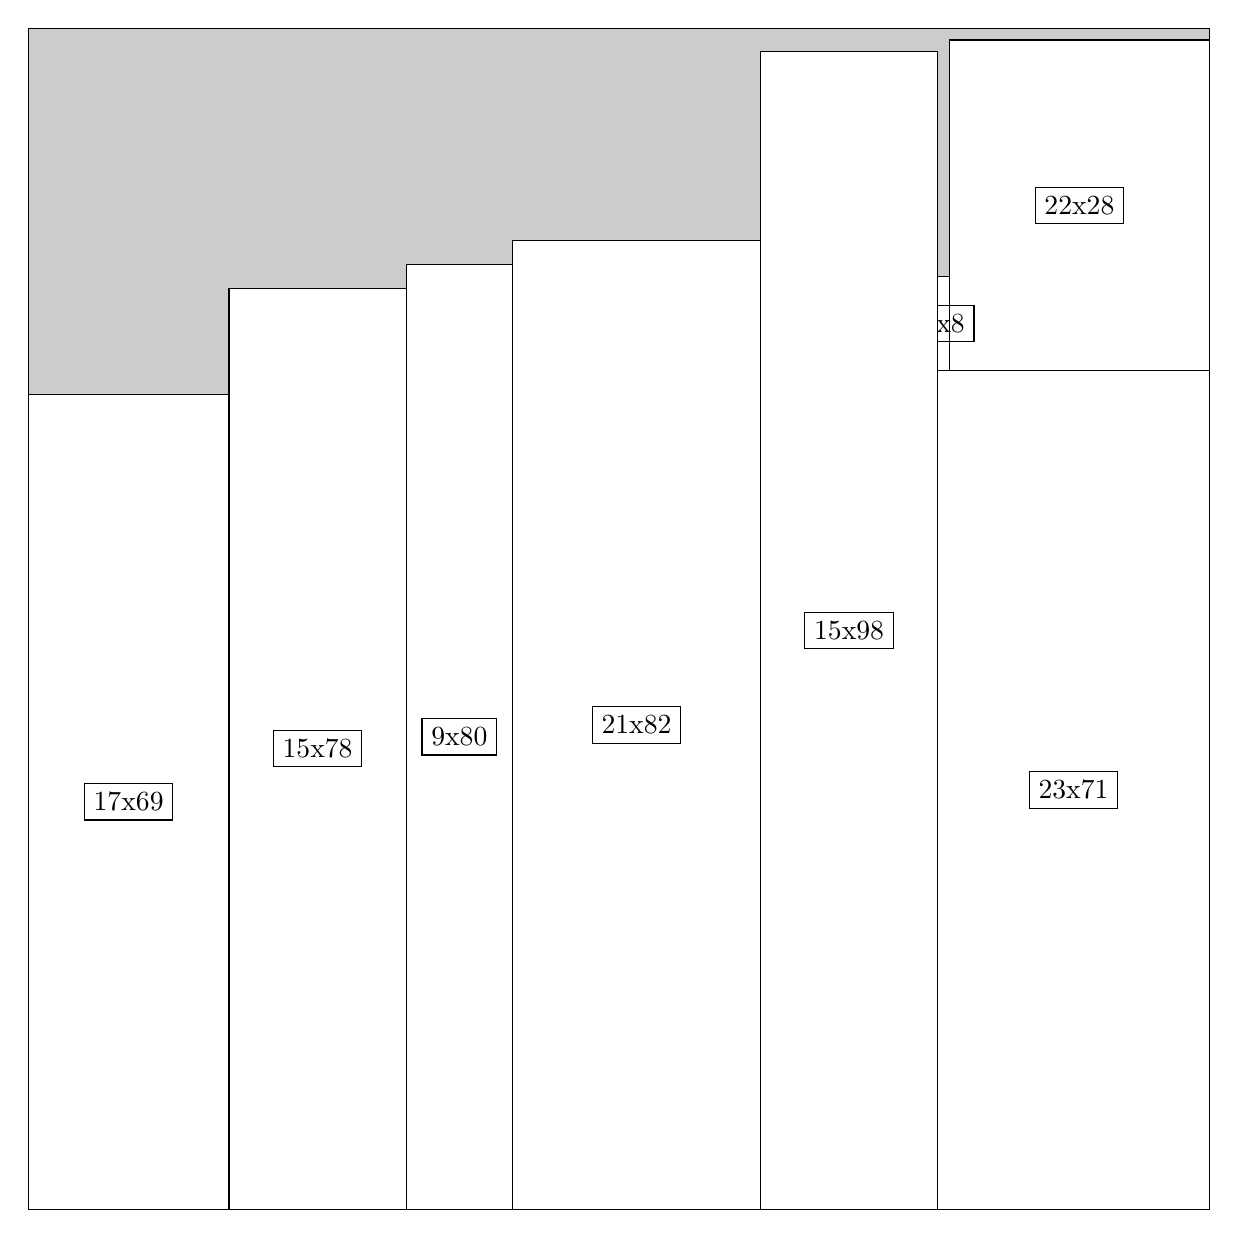
\begin{tikzpicture}[shorten >=1pt,scale=1.0,every node/.style={scale=1.0},->]
\tikzstyle{vertex}=[circle,fill=black!25,minimum size=14pt,inner sep=0pt]
\filldraw[fill=gray!40!white, draw=black] (0,0) rectangle (15.0,15.0);
\foreach \name/\x/\y/\w/\h in {23x71/11.549999999999999/0.0/3.4499999999999997/10.65,22x28/11.7/10.65/3.3/4.2,1x8/11.549999999999999/10.65/0.15/1.2,15x98/9.299999999999999/0.0/2.25/14.7,21x82/6.1499999999999995/0.0/3.15/12.299999999999999,9x80/4.8/0.0/1.3499999999999999/12.0,15x78/2.55/0.0/2.25/11.7,17x69/0.0/0.0/2.55/10.35}
\filldraw[fill=white!40!white, draw=black] (\x,\y) rectangle node[draw] (\name) {\name} ++(\w,\h);
\end{tikzpicture}


w =23 , h =71 , x =77 , y =0 , v =1633
\par
w =22 , h =28 , x =78 , y =71 , v =616
\par
w =1 , h =8 , x =77 , y =71 , v =8
\par
w =15 , h =98 , x =62 , y =0 , v =1470
\par
w =21 , h =82 , x =41 , y =0 , v =1722
\par
w =9 , h =80 , x =32 , y =0 , v =720
\par
w =15 , h =78 , x =17 , y =0 , v =1170
\par
w =17 , h =69 , x =0 , y =0 , v =1173
\par
\newpage


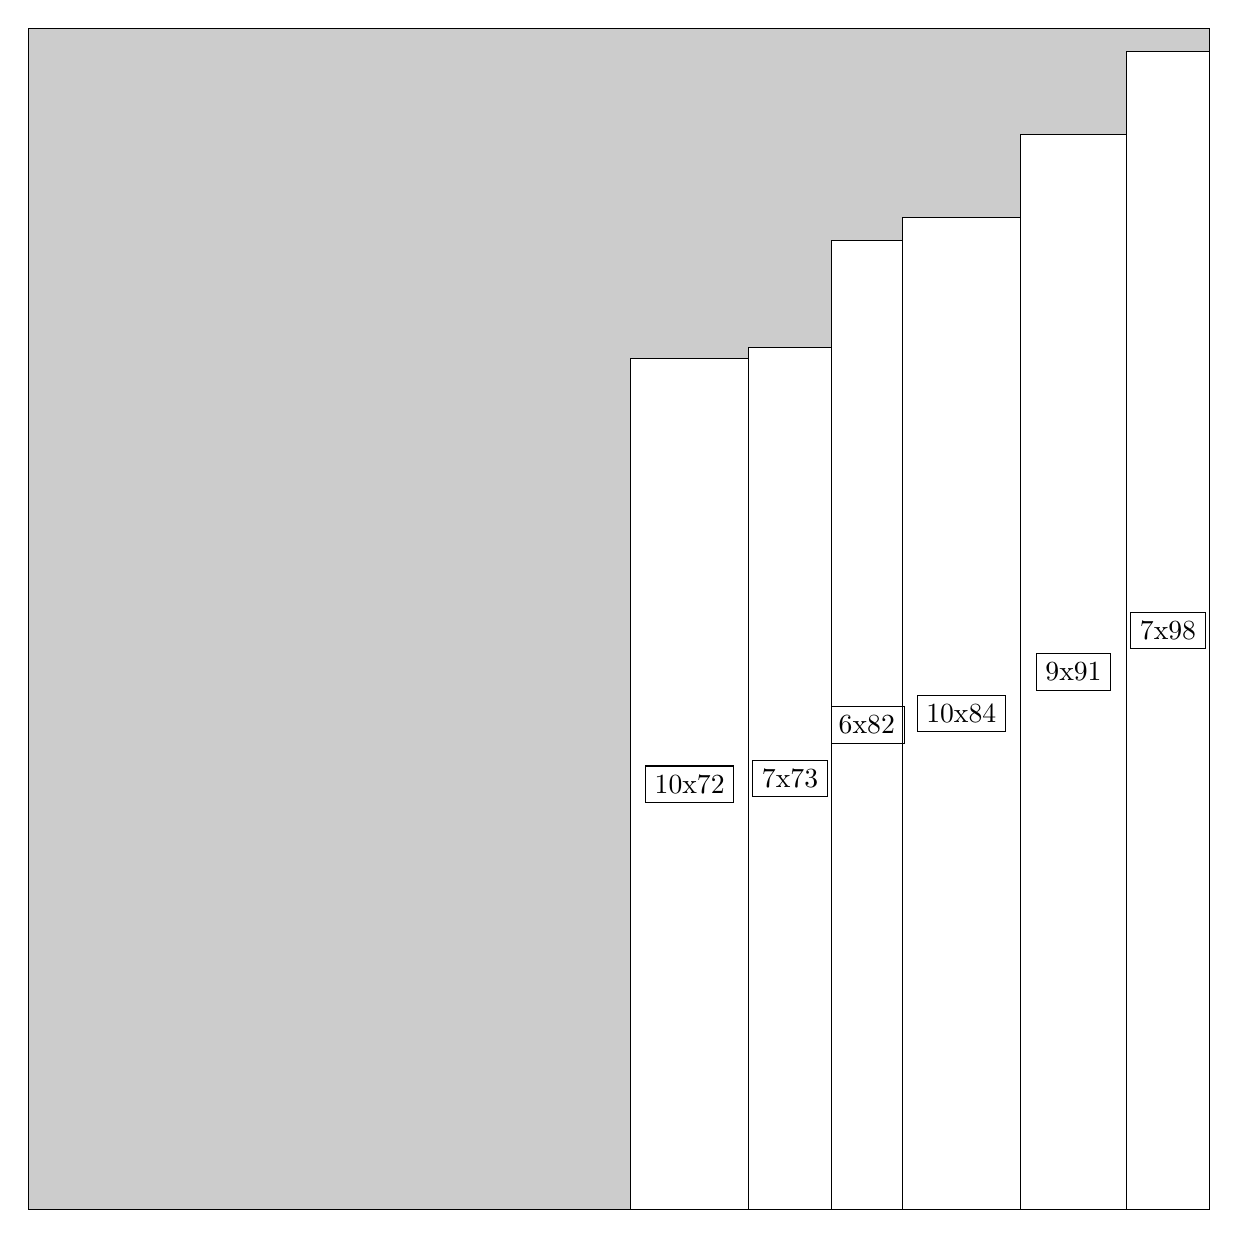
\begin{tikzpicture}[shorten >=1pt,scale=1.0,every node/.style={scale=1.0},->]
\tikzstyle{vertex}=[circle,fill=black!25,minimum size=14pt,inner sep=0pt]
\filldraw[fill=gray!40!white, draw=black] (0,0) rectangle (15.0,15.0);
\foreach \name/\x/\y/\w/\h in {7x98/13.95/0.0/1.05/14.7,9x91/12.6/0.0/1.3499999999999999/13.65,10x84/11.1/0.0/1.5/12.6,6x82/10.2/0.0/0.8999999999999999/12.299999999999999,7x73/9.15/0.0/1.05/10.95,10x72/7.6499999999999995/0.0/1.5/10.799999999999999}
\filldraw[fill=white!40!white, draw=black] (\x,\y) rectangle node[draw] (\name) {\name} ++(\w,\h);
\end{tikzpicture}


w =7 , h =98 , x =93 , y =0 , v =686
\par
w =9 , h =91 , x =84 , y =0 , v =819
\par
w =10 , h =84 , x =74 , y =0 , v =840
\par
w =6 , h =82 , x =68 , y =0 , v =492
\par
w =7 , h =73 , x =61 , y =0 , v =511
\par
w =10 , h =72 , x =51 , y =0 , v =720
\par
\newpage


\end{document}